\documentclass{article}\usepackage[]{graphicx}\usepackage[]{xcolor}
% maxwidth is the original width if it is less than linewidth
% otherwise use linewidth (to make sure the graphics do not exceed the margin)
\makeatletter
\def\maxwidth{ %
  \ifdim\Gin@nat@width>\linewidth
    \linewidth
  \else
    \Gin@nat@width
  \fi
}
\makeatother

\definecolor{fgcolor}{rgb}{0.345, 0.345, 0.345}
\newcommand{\hlnum}[1]{\textcolor[rgb]{0.686,0.059,0.569}{#1}}%
\newcommand{\hlsng}[1]{\textcolor[rgb]{0.192,0.494,0.8}{#1}}%
\newcommand{\hlcom}[1]{\textcolor[rgb]{0.678,0.584,0.686}{\textit{#1}}}%
\newcommand{\hlopt}[1]{\textcolor[rgb]{0,0,0}{#1}}%
\newcommand{\hldef}[1]{\textcolor[rgb]{0.345,0.345,0.345}{#1}}%
\newcommand{\hlkwa}[1]{\textcolor[rgb]{0.161,0.373,0.58}{\textbf{#1}}}%
\newcommand{\hlkwb}[1]{\textcolor[rgb]{0.69,0.353,0.396}{#1}}%
\newcommand{\hlkwc}[1]{\textcolor[rgb]{0.333,0.667,0.333}{#1}}%
\newcommand{\hlkwd}[1]{\textcolor[rgb]{0.737,0.353,0.396}{\textbf{#1}}}%
\let\hlipl\hlkwb

\usepackage{framed}
\makeatletter
\newenvironment{kframe}{%
 \def\at@end@of@kframe{}%
 \ifinner\ifhmode%
  \def\at@end@of@kframe{\end{minipage}}%
  \begin{minipage}{\columnwidth}%
 \fi\fi%
 \def\FrameCommand##1{\hskip\@totalleftmargin \hskip-\fboxsep
 \colorbox{shadecolor}{##1}\hskip-\fboxsep
     % There is no \\@totalrightmargin, so:
     \hskip-\linewidth \hskip-\@totalleftmargin \hskip\columnwidth}%
 \MakeFramed {\advance\hsize-\width
   \@totalleftmargin\z@ \linewidth\hsize
   \@setminipage}}%
 {\par\unskip\endMakeFramed%
 \at@end@of@kframe}
\makeatother

\definecolor{shadecolor}{rgb}{.97, .97, .97}
\definecolor{messagecolor}{rgb}{0, 0, 0}
\definecolor{warningcolor}{rgb}{1, 0, 1}
\definecolor{errorcolor}{rgb}{1, 0, 0}
\newenvironment{knitrout}{}{} % an empty environment to be redefined in TeX

\usepackage{alltt}
% \usepackage[british]{babel}
% \usepackage{csquotes}
\usepackage{natbib} % For managing references
\usepackage{listings}
\usepackage{float}
\usepackage{indentfirst}

\usepackage{geometry}
 \geometry{
 a4paper,
 margin=1in
}
\IfFileExists{upquote.sty}{\usepackage{upquote}}{}
\begin{document}

\pagenumbering{gobble}

\begin{center}
    \vspace{-1cm}  
    
\includegraphics[width=\textwidth]{images/bcu-logo.jpg}
\end{center}

\vspace{2cm}  
\noindent \Huge {\textbf{Data Visualisation Report}} \\
\normalsize \textbf{CMP5352 Semester 4}\\
\normalsize \textbf{\today}\\[1cm]

\noindent \normalsize \textbf{Word Count: 2760}\\[1cm]

\noindent \normalsize \textbf{Abhash Rai 23140736} \\
\small Abhash.Rai@mail.bcu.ac.uk \\
\small School of Computing and Digital Technology \\
\small Birmingham City University

\vfill
\hspace*{\fill}\large \textit{This work is original and independent.}\hspace*{\fill}

\restoregeometry
\pagenumbering{arabic}
\newpage


\tableofcontents
\newpage

\listoffigures
\newpage

\addcontentsline{toc}{section}{Abstract} % Add to the table of contents
\section*{Abstract}
A crucial aspect in financial industry is assessing the likelihood of a customer repaying their debt. In an era where data-driven decision-making is highly important, understanding what factors have impact on creditworthiness is vital for both lenders and borrowers.\\

This report analyzes a real-world dataset using data visualization and predictive modeling technique to examine relationships between factors like demographic characteristics, financial factors and customer characteristics and their effect on creditworthiness to answer five non-trivial research questions. The report also depicts the steps of a data science project lifecycle from data collection, data preprocessing, exploratory data analysis, feature engineering, modeling to reporting the insights.\\

The insights outlined in this report offer valuable information for financial institutions seeking to improve their risk management practices and for individuals aiming to make informed financial decisions.
\newpage


\section{Introduction}

Data visualization play a crucial role in the information society to make informed and data driven decision for both professionals and non-professionals across diverse fields \citep{inastrilla2023data}. It is a useful tool for understanding complex data to identify trends, extract insights and communicate them effectively. Humans, being visually oriented, easily understand compelling stories of abstract data when transformed into visualizations \citep{qin2020making}. \cite{shakeel2022comprehensive} states people have natural affinity for effective visual representation. \\

This report focuses on analyzing a real-world `Credit Card Eligibility Dataset' obtained from Kaggle to provide answer and justification to several non-trivial research questions. The aim of the report is to identify and analyze key factors influencing credit card eligibility and financial well-being of individuals, and present the findings in a clear and compelling manner. \\

The report is structured in four sections. An explanation of the selected dataset and reasoning for its selection is provided in the `Motivation and Objectives' section, along with the non-trivial research questions, each justified for its complexity and significance. Then, `Dataset Wrangling' section outlines the wrangling steps taken including code to clean the dataset which is then used for exploratory data analysis. Following that, the `Experimental Results' section summarizes the results using high-quality graphs, each of which has a brief caption addressing the non-trivial research questions. Finally, the `Conclusion' section concludes by going over the questions, outlining the key takeaways from the research, and drawing conclusions. 
\newpage

\section{Motivation and Objectives}

\subsection{Dataset Selection}

Accurate assessment of credit risk is important, especially in case of financial services industry. In order to minimize the risk of default, financial institutions have to establish a credit risk management framework for taking informed decisions when issuing credit cards. This report provides the research and analysis work on `Credit Card Eligibility Dataset' which can be utilized to address such challenges. \\

The dataset is publicly available and contains a rich set of variables which was among the reason for its selection. The dataset was primarily selected to potentially provide financial providers and customers understanding of factors which impact financial well-being of individuals and aid in making informed decision like credit card issuance.

\subsection{Dataset Overview}

The `Credit Card Eligibility Dataset', sourced from Kaggle, contains information about customer demographics, financial status, employment details, lifestyle and credit risk status. The dataset contains discrete, continuous, and categorical data. It has 36457 rows and 18 columns. The columns are:

\begin{enumerate}
\item Gender
\item Has.a.car
\item Has.a.property
\item Children.count
\item Income
\item Employment.status
\item Education.level
\item Marital.status
\item Dwelling
\item Customer.relative.age
\item Employment.relative.length
\item Has.a.work.phone
\item Has.a.phone
\item Has.an.email
\item Job.title
\item Family.member.count
\item Account.relative.age
\item Is.high.risk\\
\end{enumerate}


In the dataset, columns like age and employment length contain negative values to serve as large reference points in the dataset rather than actual values. With age, a negative value, for example, -30, means that the person is 30 units younger since a specific reference date, so essentially, the number of units the account has been around, but counted backwards from now. Also, employment length is measured from the present day and positive numbers mean unemployment periods.

\subsection{Non-Trivial Research Questions}

The non-trivial research questions explored in this report are outlined below with brief description and justification as to why they are non-trivial for every question.\\

\begin{enumerate}
\item \textbf{What factors greatly contribute to risk status of customers for credit card?} \\ This question focuses on factors which directly affect the classificaiton of customers as either high risk or low risk. Finding the most influential features contributing to credit risk is highly informative. The goal is to rank these features based on their impact on credit risk status which can help financial institutions to improve risk assessment and develop strategies to enhancing financial stability.\\
\item \textbf{Which professions have a higher chance of being classified as high risk?} \\ This question examines proportions of high-risk individuals associated with job titles, finding any jobs that may disproportionately contribute to the high-risk pool. Identifying these trends helps lenders refine risk models and offer tailored financial advice to at-risk professional groups.\\
\item \textbf{How does employment duration and status influence income levels among customers?} \\ This question is aimed to investigate the association among the work experience length, work status, and income levels. Duration of employment indicates job security and career advancement and status in turn may very well impact earning capabilities. This is an important question due to personal career trajectories in a fast-moving labour market. Insights can then help inform policymakers, financial planners  in addressing income disparity and job market policies.\\
\item \textbf{Does asset ownership significantly impact income levels, and does this impact differ between high-risk and low-risk customers?} \\ This question studies whether the ownership of assets determines levels of income and if this impact varies between high-risk and low-risk customers. Results can be used to inform strategies from financial providers to design products that support asset growth and income stability, especially for high credit risk customers, by tailoring offerings like secured loans or asset-backed credit lines.\\
\item \textbf{Does higher education level mean high income?} \\ This research explores the relationship between education level and income. While higher education is assumed to lead to higher earnings, the study quantifies this relationship and examines exceptions. These insights can help individuals make informed educational investments.\\
\end{enumerate}
\newpage






\section{Dataset Wrangling}

\subsection{Data Preprocessing}

\begin{knitrout}
\definecolor{shadecolor}{rgb}{0.969, 0.969, 0.969}\color{fgcolor}\begin{kframe}
\begin{alltt}
\hlcom{#install.packages("tidyverse")}
\hlkwd{library}\hldef{(tidyverse)}
\hldef{df} \hlkwb{<-} \hlkwd{read.csv}\hldef{(}\hlsng{"credit_eligibility.csv"}\hldef{)}
\hlkwd{names}\hldef{(df)}
\end{alltt}
\begin{verbatim}
##  [1] "ID"                  "Gender"              "Has.a.car"          
##  [4] "Has.a.property"      "Children.count"      "Income"             
##  [7] "Employment.status"   "Education.level"     "Marital.status"     
## [10] "Dwelling"            "Age"                 "Employment.length"  
## [13] "Has.a.mobile.phone"  "Has.a.work.phone"    "Has.a.phone"        
## [16] "Has.an.email"        "Job.title"           "Family.member.count"
## [19] "Account.age"         "Is.high.risk"
\end{verbatim}
\begin{alltt}
\hlkwd{dim}\hldef{(df)}
\end{alltt}
\begin{verbatim}
## [1] 36457    20
\end{verbatim}
\end{kframe}
\end{knitrout}

The dataset was first loaded into variable `df' for initiating the data wrangling process. 

\begin{knitrout}
\definecolor{shadecolor}{rgb}{0.969, 0.969, 0.969}\color{fgcolor}\begin{kframe}
\begin{alltt}
\hlkwd{problems}\hldef{(df)}
\hlkwd{str}\hldef{(df)}
\hlkwd{summary}\hldef{(df)}
\end{alltt}
\end{kframe}
\end{knitrout}

Initial exploration of the dataset was performed by identifying potential issues, summarizing the structure and statistical properties of the data. Some columns represent relative units which should be set to have accurate names to prevent any misinterpretation. On a closer look, the dataset contains boolean features such as `Gender', `Has.a.car' and `Has.a.property' which have values either `Y' or `N'. Similarly, other boolean feature columns `Has.a.mobile.phone', `Has.a.work.phone', `Has.a.phone', `Has.an.email' and `Is.high.risk' have values `0' or `1'. So these columns must be handled appropriately to set the correct values.

\begin{knitrout}
\definecolor{shadecolor}{rgb}{0.969, 0.969, 0.969}\color{fgcolor}\begin{kframe}
\begin{alltt}
\hldef{df} \hlkwb{<-} \hldef{df} \hlopt \hlkwd{select}\hldef{(}\hlopt{-}\hldef{ID)}
\end{alltt}
\end{kframe}
\end{knitrout}

The `ID' column was removed as it does not provide any significant impact during analysis.

\begin{knitrout}
\definecolor{shadecolor}{rgb}{0.969, 0.969, 0.969}\color{fgcolor}\begin{kframe}
\begin{alltt}
\hlcom{# Some columns represent durations measured relative to a reference point}
\hlcom{# Giving those columns an appropriate name}
\hlkwd{names}\hldef{(df)[}\hlkwd{names}\hldef{(df)} \hlopt{==} \hlsng{"Age"}\hldef{]} \hlkwb{<-} \hlsng{"Customer.relative.age"}
\hlkwd{names}\hldef{(df)[}\hlkwd{names}\hldef{(df)} \hlopt{==} \hlsng{"Account.age"}\hldef{]} \hlkwb{<-} \hlsng{"Account.relative.age"}
\hlkwd{names}\hldef{(df)[}\hlkwd{names}\hldef{(df)} \hlopt{==} \hlsng{"Employment.length"}\hldef{]} \hlkwb{<-} \hlsng{"Employment.relative.length"}
\end{alltt}
\end{kframe}
\end{knitrout}

The relative unit columns were assigned proper names.

\begin{knitrout}
\definecolor{shadecolor}{rgb}{0.969, 0.969, 0.969}\color{fgcolor}\begin{kframe}
\begin{alltt}
\hldef{df} \hlkwb{<-} \hldef{df} \hlopt
  \hlkwd{mutate}\hldef{(}\hlkwc{Gender} \hldef{=} \hlkwd{ifelse}\hldef{(Gender} \hlopt{==} \hlsng{"M"}\hldef{,} \hlsng{"Male"}\hldef{,} \hlsng{"Female"}\hldef{))}
\end{alltt}
\end{kframe}
\end{knitrout}

The `Gender' column was assigned proper values: `Male' and `Female'.

\begin{knitrout}
\definecolor{shadecolor}{rgb}{0.969, 0.969, 0.969}\color{fgcolor}\begin{kframe}
\begin{alltt}
\hldef{df} \hlkwb{<-} \hldef{df} \hlopt
  \hlkwd{mutate}\hldef{(}
    \hlkwc{Has.a.car} \hldef{=} \hlkwd{ifelse}\hldef{(Has.a.car} \hlopt{==} \hlsng{"Y"}\hldef{,} \hlnum{TRUE}\hldef{,} \hlnum{FALSE}\hldef{),}
    \hlkwc{Has.a.property} \hldef{=} \hlkwd{ifelse}\hldef{(Has.a.property} \hlopt{==} \hlsng{"Y"}\hldef{,} \hlnum{TRUE}\hldef{,} \hlnum{FALSE}\hldef{),}
    \hlkwc{Has.a.work.phone} \hldef{=} \hlkwd{ifelse}\hldef{(Has.a.work.phone} \hlopt{==} \hlnum{1}\hldef{,} \hlnum{TRUE}\hldef{,} \hlnum{FALSE}\hldef{),}
    \hlkwc{Has.a.phone} \hldef{=} \hlkwd{ifelse}\hldef{(Has.a.phone} \hlopt{==} \hlnum{1}\hldef{,} \hlnum{TRUE}\hldef{,} \hlnum{FALSE}\hldef{),}
    \hlkwc{Has.an.email} \hldef{=} \hlkwd{ifelse}\hldef{(Has.an.email} \hlopt{==} \hlnum{1}\hldef{,} \hlnum{TRUE}\hldef{,} \hlnum{FALSE}\hldef{),}
    \hlkwc{Is.high.risk} \hldef{=} \hlkwd{ifelse}\hldef{(Is.high.risk} \hlopt{==} \hlnum{1}\hldef{,} \hlnum{TRUE}\hldef{,} \hlnum{FALSE}\hldef{)}
\hldef{)}
\end{alltt}
\end{kframe}
\end{knitrout}

The binary features in the dataset were modified to have boolean values `True' or `False' and data type set to logical.

\begin{knitrout}
\definecolor{shadecolor}{rgb}{0.969, 0.969, 0.969}\color{fgcolor}\begin{kframe}
\begin{alltt}
\hldef{df}\hlopt{$}\hldef{Family.member.count} \hlkwb{<-} \hlkwd{as.integer}\hldef{(}
  \hldef{df}\hlopt{$}\hldef{Family.member.count)}
\hldef{df}\hlopt{$}\hldef{Account.relative.age} \hlkwb{<-} \hlkwd{as.numeric}\hldef{(}
  \hldef{df}\hlopt{$}\hldef{Account.relative.age)}
\hldef{df}\hlopt{$}\hldef{Employment.relative.length} \hlkwb{<-} \hlkwd{as.numeric}\hldef{(}
  \hldef{df}\hlopt{$}\hldef{Employment.relative.length)}
\hldef{df}\hlopt{$}\hldef{Customer.relative.age} \hlkwb{<-} \hlkwd{as.numeric}\hldef{(}
  \hldef{df}\hlopt{$}\hldef{Customer.relative.age)}
\end{alltt}
\end{kframe}
\end{knitrout}

The data types of above columns were set to `integer' and `numeric' based on their nature.

\begin{knitrout}
\definecolor{shadecolor}{rgb}{0.969, 0.969, 0.969}\color{fgcolor}\begin{kframe}
\begin{alltt}
\hlkwd{unique}\hldef{(df}\hlopt{$}\hldef{Has.a.mobile.phone)}
\end{alltt}
\begin{verbatim}
## [1] 1
\end{verbatim}
\begin{alltt}
\hldef{df} \hlkwb{<-} \hldef{df} \hlopt \hlkwd{select}\hldef{(}\hlopt{-}\hldef{Has.a.mobile.phone)}
\end{alltt}
\end{kframe}
\end{knitrout}

`Has.a.mobile.phone' column has only a single value. So, it was removed.

\begin{knitrout}
\definecolor{shadecolor}{rgb}{0.969, 0.969, 0.969}\color{fgcolor}\begin{kframe}
\begin{alltt}
\hldef{df} \hlkwb{<-} \hldef{df} \hlopt
  \hlkwd{mutate}\hldef{(}\hlkwd{across}\hldef{(}\hlkwd{where}\hldef{(is.character),} \hlopt{~} \hlkwd{str_to_title}\hldef{(}\hlkwd{as.character}\hldef{(.))))}
\end{alltt}
\end{kframe}
\end{knitrout}

The values of categorical columns were transformed to title case in the dataframe.

\begin{knitrout}
\definecolor{shadecolor}{rgb}{0.969, 0.969, 0.969}\color{fgcolor}\begin{kframe}
\begin{alltt}
\hlkwd{dim}\hldef{(df)}
\end{alltt}
\begin{verbatim}
## [1] 36457    18
\end{verbatim}
\end{kframe}
\end{knitrout}
















\subsection{Exploratory Data Analysis}

\subsubsection{Null Values}

\begin{knitrout}
\definecolor{shadecolor}{rgb}{0.969, 0.969, 0.969}\color{fgcolor}\begin{kframe}
\begin{alltt}
\hldef{df[df} \hlopt{==} \hlsng{""}\hldef{]} \hlkwb{<-} \hlnum{NA} \hlcom{# Converting empty strings to NA values}
\hldef{result} \hlkwb{<-} \hlkwd{colSums}\hldef{(}\hlkwd{is.na}\hldef{(df))}
\hldef{result_df} \hlkwb{<-} \hlkwd{data.frame}\hldef{(}\hlkwc{Column_Names} \hldef{=} \hlkwd{names}\hldef{(result),} \hlkwc{NA_Count} \hldef{= result)}
\hlkwd{rownames}\hldef{(result_df)} \hlkwb{<-} \hlkwa{NULL}
\hldef{result_df}
\end{alltt}
\begin{verbatim}
##                  Column_Names NA_Count
## 1                      Gender        0
## 2                   Has.a.car        0
## 3              Has.a.property        0
## 4              Children.count        0
## 5                      Income        0
## 6           Employment.status        0
## 7             Education.level        0
## 8              Marital.status        0
## 9                    Dwelling        0
## 10      Customer.relative.age        0
## 11 Employment.relative.length        0
## 12           Has.a.work.phone        0
## 13                Has.a.phone        0
## 14               Has.an.email        0
## 15                  Job.title    11323
## 16        Family.member.count        0
## 17       Account.relative.age        0
## 18               Is.high.risk        0
\end{verbatim}
\end{kframe}
\end{knitrout}

Only `Job.title' column contains null values with a total null value count of 11323.


\subsubsection{Categorical Features}

\begin{knitrout}
\definecolor{shadecolor}{rgb}{0.969, 0.969, 0.969}\color{fgcolor}\begin{kframe}
\begin{alltt}
\hldef{character_columns} \hlkwb{<-} \hldef{df} \hlopt \hlkwd{select_if}\hldef{(is.character)}
\hlkwd{names}\hldef{(character_columns)}
\end{alltt}
\begin{verbatim}
## [1] "Gender"            "Employment.status" "Education.level"  
## [4] "Marital.status"    "Dwelling"          "Job.title"
\end{verbatim}
\end{kframe}
\end{knitrout}

To explore above listed categorical columns two custom functions were defined: one for visualizing data distribution of the feature, and another for analyzing the feature.

\begin{knitrout}
\definecolor{shadecolor}{rgb}{0.969, 0.969, 0.969}\color{fgcolor}\begin{kframe}
\begin{alltt}
\hlcom{# install.packages("ggplot2")}
\hlcom{# install.packages("ggrepel")}
\hlkwd{library}\hldef{(ggplot2)}
\hlkwd{library}\hldef{(ggrepel)}

\hldef{create_pie_chart_for_category} \hlkwb{<-} \hlkwa{function}\hldef{(}\hlkwc{df}\hldef{,} \hlkwc{column}\hldef{) \{}

  \hldef{df_clean} \hlkwb{<-} \hldef{df[}\hlopt{!}\hlkwd{is.na}\hldef{(df[[column]]), ]}

  \hldef{value_count_df} \hlkwb{<-} \hlkwd{data.frame}\hldef{(}\hlkwd{table}\hldef{(df_clean[[column]]))}
  \hlkwd{colnames}\hldef{(value_count_df)} \hlkwb{<-} \hlkwd{c}\hldef{(}\hlsng{"group"}\hldef{,} \hlsng{"value"}\hldef{)}

  \hldef{value_count_df} \hlkwb{<-} \hldef{value_count_df[value_count_df}\hlopt{$}\hldef{value} \hlopt{!=} \hlnum{0}\hldef{, ]}

  \hldef{label_position} \hlkwb{<-} \hldef{value_count_df} \hlopt
    \hlkwd{mutate}\hldef{(}\hlkwc{csum} \hldef{=} \hlkwd{rev}\hldef{(}\hlkwd{cumsum}\hldef{(}\hlkwd{rev}\hldef{(value))),}
           \hlkwc{pos} \hldef{= value}\hlopt{/}\hlnum{2} \hlopt{+} \hlkwd{lead}\hldef{(csum,} \hlnum{1}\hldef{),}
           \hlkwc{pos} \hldef{=} \hlkwd{if_else}\hldef{(}\hlkwd{is.na}\hldef{(pos), value}\hlopt{/}\hlnum{2}\hldef{, pos))}

  \hlkwd{ggplot}\hldef{(}
    \hldef{value_count_df,}
    \hlkwd{aes}\hldef{(}\hlkwc{x} \hldef{=} \hlsng{""} \hldef{,} \hlkwc{y} \hldef{= value,} \hlkwc{fill} \hldef{=} \hlkwd{fct_inorder}\hldef{(group)))} \hlopt{+}
    \hlkwd{geom_col}\hldef{(}\hlkwc{width} \hldef{=} \hlnum{1}\hldef{,} \hlkwc{color} \hldef{=} \hlnum{1}\hldef{)} \hlopt{+}
    \hlkwd{coord_polar}\hldef{(}\hlkwc{theta} \hldef{=} \hlsng{"y"}\hldef{)} \hlopt{+}
    \hlkwd{scale_fill_brewer}\hldef{(}\hlkwc{palette} \hldef{=} \hlsng{"Accent"}\hldef{)} \hlopt{+}
    \hlkwd{geom_label_repel}\hldef{(}
      \hlkwc{data} \hldef{= label_position,}
      \hlkwd{aes}\hldef{(}
        \hlkwc{y} \hldef{= pos,}
        \hlkwc{label} \hldef{=} \hlkwd{paste0}\hldef{(}
          \hlkwd{round}\hldef{((value}\hlopt{/}\hlkwd{sum}\hldef{(value_count_df}\hlopt{$}\hldef{value))}\hlopt{*}\hlnum{100}\hldef{,} \hlnum{2}\hldef{),} \hlsng{"%"}
        \hldef{)}
      \hldef{),}
      \hlkwc{size} \hldef{=} \hlnum{4.5}\hldef{,} \hlkwc{nudge_x} \hldef{=} \hlnum{1}\hldef{,} \hlkwc{show.legend} \hldef{=} \hlnum{FALSE}
    \hldef{)} \hlopt{+}
    \hlkwd{guides}\hldef{(}\hlkwc{fill} \hldef{=} \hlkwd{guide_legend}\hldef{(}\hlkwc{title} \hldef{=} \hlsng{""}\hldef{))} \hlopt{+}
    \hlkwd{theme_void}\hldef{()} \hlopt{+}
    \hlkwd{ggtitle}\hldef{(}\hlkwd{paste0}\hldef{(}\hlsng{"Distribution of "}\hldef{, column))} \hlopt{+}
    \hlkwd{theme}\hldef{(}
      \hlkwc{plot.title} \hldef{=} \hlkwd{element_text}\hldef{(}
        \hlkwc{hjust} \hldef{=} \hlnum{0.5}\hldef{,} \hlkwc{margin} \hldef{=} \hlkwd{margin}\hldef{(}\hlkwc{t} \hldef{=} \hlnum{0}\hldef{,} \hlkwc{b} \hldef{=} \hlnum{10}\hldef{),} \hlkwc{face} \hldef{=} \hlsng{"bold"}
      \hldef{)}
    \hldef{)}
\hldef{\}}
\end{alltt}
\end{kframe}
\end{knitrout}

Above function used `ggplot2' and `ggrepel' to create pie charts, given a dataframe and the column name as parameter respectively.

\begin{knitrout}
\definecolor{shadecolor}{rgb}{0.969, 0.969, 0.969}\color{fgcolor}\begin{kframe}
\begin{alltt}
\hldef{analyze_character_column} \hlkwb{<-} \hlkwa{function}\hldef{(}\hlkwc{df}\hldef{,} \hlkwc{col_name}\hldef{) \{}

  \hlkwa{if} \hldef{(}\hlopt{!}\hldef{col_name} \hlopt \hlkwd{names}\hldef{(df)) \{}
    \hlkwd{stop}\hldef{(}\hlsng{"Column '"}\hldef{, col_name,} \hlsng{"' not found in the data frame."}\hldef{)}
  \hldef{\}}

  \hldef{df_clean} \hlkwb{<-} \hldef{df[}\hlopt{!}\hlkwd{is.na}\hldef{(df[[col_name]]), ]}
  \hldef{column_data} \hlkwb{<-} \hldef{df_clean[[col_name]]}

  \hlkwa{if} \hldef{(}\hlopt{!}\hlkwd{is.character}\hldef{(column_data)) \{}
    \hlkwd{stop}\hldef{(}\hlsng{"Column '"}\hldef{, col_name,} \hlsng{"' is not of character type."}\hldef{)}
  \hldef{\}}

  \hlkwd{cat}\hldef{(}\hlsng{"Column:"}\hldef{, col_name,} \hlsng{"\textbackslash{}n"}\hldef{)}
  \hldef{unique_vals} \hlkwb{<-} \hlkwd{unique}\hldef{(column_data)}
  \hldef{num_unique_vals} \hlkwb{<-} \hlkwd{length}\hldef{(unique_vals)}
  \hlkwd{cat}\hldef{(}\hlsng{"Number of unique values:"}\hldef{, num_unique_vals,} \hlsng{"\textbackslash{}n"}\hldef{)}
  \hlkwd{cat}\hldef{(}\hlsng{"Value counts:\textbackslash{}n"}\hldef{)}

  \hldef{value_count_df} \hlkwb{<-} \hlkwd{data.frame}\hldef{(}\hlkwd{table}\hldef{(column_data))}
  \hlkwd{colnames}\hldef{(value_count_df)} \hlkwb{<-} \hlkwd{c}\hldef{(}\hlsng{"Category"}\hldef{,} \hlsng{"Count"}\hldef{)}
  \hldef{value_count_df}\hlopt{$}\hldef{Percentage} \hlkwb{<-} \hlkwd{round}\hldef{(}
    \hldef{(value_count_df}\hlopt{$}\hldef{Count} \hlopt{/} \hlkwd{sum}\hldef{(value_count_df}\hlopt{$}\hldef{Count))} \hlopt{*} \hlnum{100}\hldef{,} \hlnum{2}
  \hldef{)}
  \hldef{value_count_df} \hlkwb{<-} \hldef{value_count_df[}
    \hlkwd{order}\hldef{(value_count_df}\hlopt{$}\hldef{Percentage,} \hlkwc{decreasing} \hldef{=} \hlnum{TRUE}\hldef{),}
  \hldef{]}
  \hlkwd{rownames}\hldef{(value_count_df)} \hlkwb{<-} \hlkwa{NULL}
  \hlkwd{print}\hldef{(value_count_df)}
  \hlkwd{cat}\hldef{(}\hlsng{"\textbackslash{}n"}\hldef{)}
\hldef{\}}
\end{alltt}
\end{kframe}
\end{knitrout}

Above second function analyzes a specified character column in a data frame, printing unique values, their counts, and their percentage distributions.

\begin{figure}[H] % [H] ensures figure is placed exactly here
\centering
\begin{knitrout}
\definecolor{shadecolor}{rgb}{0.969, 0.969, 0.969}\color{fgcolor}\begin{kframe}
\begin{alltt}
\hlkwd{create_pie_chart_for_category}\hldef{(df,} \hlsng{"Gender"}\hldef{)}
\end{alltt}
\end{kframe}
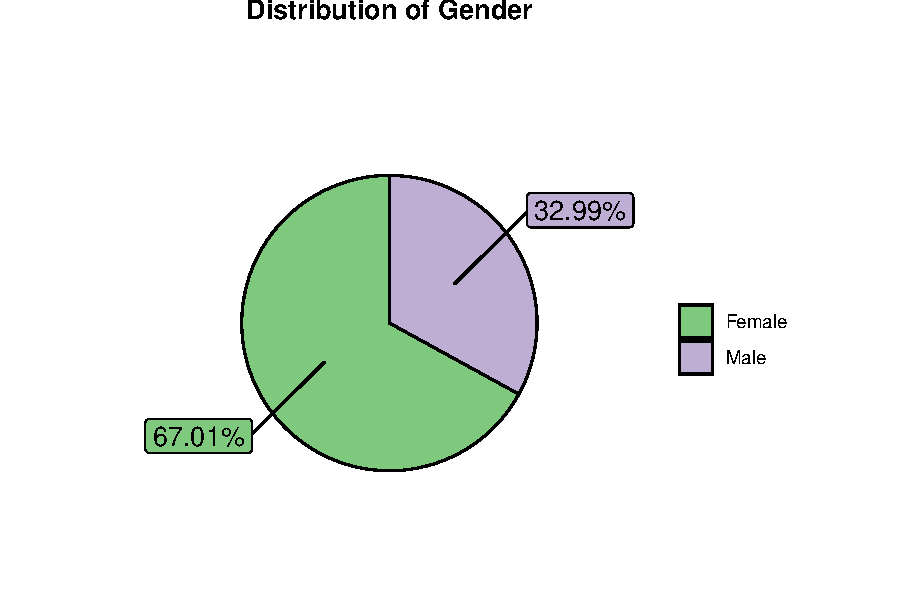
\includegraphics[width=\maxwidth]{figure/unnamed-chunk-15-1} 
\end{knitrout}
\vspace{-40pt} % Reducing space
\caption{Distribution of Gender}
\end{figure}

\begin{knitrout}
\definecolor{shadecolor}{rgb}{0.969, 0.969, 0.969}\color{fgcolor}\begin{kframe}
\begin{alltt}
\hlkwd{analyze_character_column}\hldef{(df,} \hlsng{"Gender"}\hldef{)}
\end{alltt}
\begin{verbatim}
## Column: Gender 
## Number of unique values: 2 
## Value counts:
##   Category Count Percentage
## 1   Female 24430      67.01
## 2     Male 12027      32.99
\end{verbatim}
\end{kframe}
\end{knitrout}

The dataset containes data of significantly more male as compared with female customers.

\begin{figure}[H] % [H] ensures figure is placed exactly here
\centering
\begin{knitrout}
\definecolor{shadecolor}{rgb}{0.969, 0.969, 0.969}\color{fgcolor}\begin{kframe}
\begin{alltt}
\hlkwd{ggplot}\hldef{(df,} \hlkwd{aes}\hldef{(}\hlkwc{x} \hldef{= Employment.status,} \hlkwc{fill} \hldef{= Employment.status))} \hlopt{+}
  \hlkwd{geom_bar}\hldef{()} \hlopt{+}
  \hlkwd{geom_text}\hldef{(}\hlkwc{stat} \hldef{=} \hlsng{"count"}\hldef{,} \hlkwd{aes}\hldef{(}\hlkwc{label} \hldef{= ..count..),} \hlkwc{vjust} \hldef{=} \hlopt{-}\hlnum{0.5}\hldef{)} \hlopt{+}
  \hlkwd{theme_classic}\hldef{()} \hlopt{+}
  \hlkwd{xlab}\hldef{(}\hlsng{"Employment Status"}\hldef{)} \hlopt{+}
  \hlkwd{ylab}\hldef{(}\hlsng{"Count"}\hldef{)} \hlopt{+}
  \hlkwd{ggtitle}\hldef{(}\hlsng{"Distribution of Employment Status"}\hldef{)} \hlopt{+}
  \hlkwd{scale_fill_brewer}\hldef{(}\hlkwc{palette} \hldef{=} \hlsng{"Set2"}\hldef{)} \hlopt{+}
  \hlkwd{theme}\hldef{(}
    \hlkwc{plot.title} \hldef{=} \hlkwd{element_text}\hldef{(}\hlkwc{hjust} \hldef{=} \hlnum{0.5}\hldef{,} \hlkwc{face} \hldef{=} \hlsng{"bold"}\hldef{,} \hlkwc{margin} \hldef{=} \hlkwd{margin}\hldef{(}\hlkwc{b} \hldef{=} \hlnum{10}\hldef{)),}
    \hlkwc{legend.position} \hldef{=} \hlsng{"bottom"}\hldef{,}
    \hlkwc{legend.title} \hldef{=} \hlkwd{element_blank}\hldef{()}
  \hldef{)} \hlopt{+}
  \hlkwd{coord_cartesian}\hldef{(}\hlkwc{ylim} \hldef{=} \hlkwd{c}\hldef{(}\hlnum{0}\hldef{,} \hlnum{20000}\hldef{))}
\end{alltt}
\end{kframe}
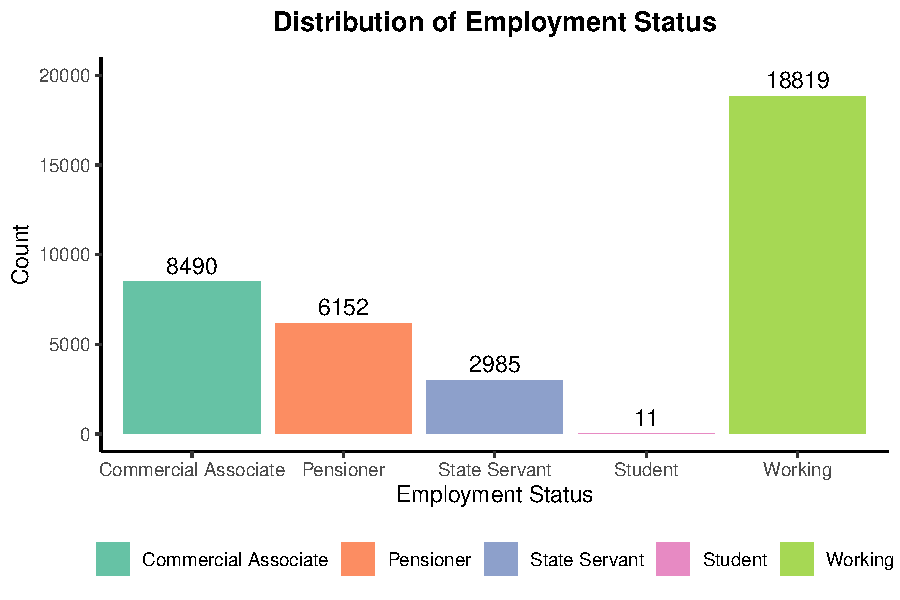
\includegraphics[width=\maxwidth]{figure/unnamed-chunk-17-1} 
\end{knitrout}
\vspace{-10pt} % Reducing space
\caption{Distribution of Customer Employment Status}
\end{figure}

\begin{knitrout}
\definecolor{shadecolor}{rgb}{0.969, 0.969, 0.969}\color{fgcolor}\begin{kframe}
\begin{alltt}
\hlkwd{analyze_character_column}\hldef{(df,} \hlsng{"Employment.status"}\hldef{)}
\end{alltt}
\begin{verbatim}
## Column: Employment.status 
## Number of unique values: 5 
## Value counts:
##               Category Count Percentage
## 1              Working 18819      51.62
## 2 Commercial Associate  8490      23.29
## 3            Pensioner  6152      16.87
## 4        State Servant  2985       8.19
## 5              Student    11       0.03
\end{verbatim}
\end{kframe}
\end{knitrout}

There are total of five categories within the employment status of the customers. Half of the customers are employed and working. The customers with lowest count in the dataset are students.

\begin{figure}[H] % [H] ensures figure is placed exactly here
\centering
\begin{knitrout}
\definecolor{shadecolor}{rgb}{0.969, 0.969, 0.969}\color{fgcolor}\begin{kframe}
\begin{alltt}
\hlkwd{create_pie_chart_for_category}\hldef{(df,} \hlsng{"Education.level"}\hldef{)}
\end{alltt}
\end{kframe}
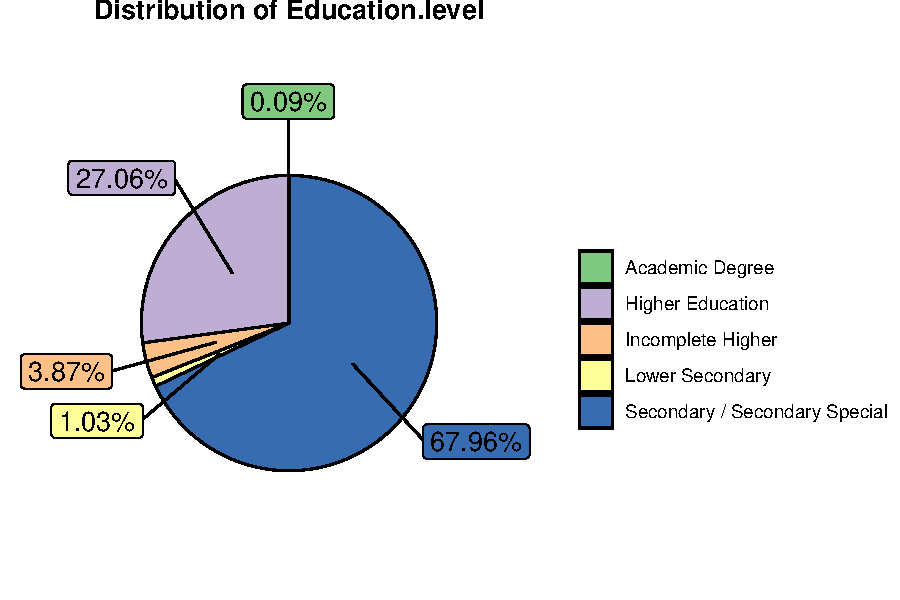
\includegraphics[width=\maxwidth]{figure/unnamed-chunk-19-1} 
\end{knitrout}
\vspace{-40pt} % Reducing space
\caption{Distribution of Education Level of Customers}
\end{figure}

\begin{knitrout}
\definecolor{shadecolor}{rgb}{0.969, 0.969, 0.969}\color{fgcolor}\begin{kframe}
\begin{alltt}
\hlkwd{analyze_character_column}\hldef{(df,} \hlsng{"Education.level"}\hldef{)}
\end{alltt}
\begin{verbatim}
## Column: Education.level 
## Number of unique values: 5 
## Value counts:
##                        Category Count Percentage
## 1 Secondary / Secondary Special 24777      67.96
## 2              Higher Education  9864      27.06
## 3             Incomplete Higher  1410       3.87
## 4               Lower Secondary   374       1.03
## 5               Academic Degree    32       0.09
\end{verbatim}
\end{kframe}
\end{knitrout}

The vast majority of customers have pursued education up to at least the secondary level or higher. There are some customer who pursed high education but dropped out before completion.


\begin{figure}[H] % [H] ensures figure is placed exactly here
\centering
\begin{knitrout}
\definecolor{shadecolor}{rgb}{0.969, 0.969, 0.969}\color{fgcolor}\begin{kframe}
\begin{alltt}
\hldef{marital_counts} \hlkwb{<-} \hlkwd{table}\hldef{(df}\hlopt{$}\hldef{Marital.status)}
\hldef{marital_df} \hlkwb{<-} \hlkwd{as.data.frame}\hldef{(marital_counts)}
\hlkwd{names}\hldef{(marital_df)} \hlkwb{<-} \hlkwd{c}\hldef{(}\hlsng{"Marital.status"}\hldef{,} \hlsng{"Count"}\hldef{)}

\hlkwd{ggplot}\hldef{(marital_df,} \hlkwd{aes}\hldef{(}\hlkwc{x} \hldef{=} \hlkwd{reorder}\hldef{(Marital.status, Count),} \hlkwc{y} \hldef{= Count))} \hlopt{+}
  \hlkwd{geom_point}\hldef{(}\hlkwd{aes}\hldef{(}\hlkwc{size} \hldef{= Count),} \hlkwc{color} \hldef{=} \hlsng{"steelblue"}\hldef{)} \hlopt{+}
  \hlkwd{geom_text}\hldef{(}\hlkwd{aes}\hldef{(}\hlkwc{label} \hldef{= Count),} \hlkwc{vjust} \hldef{=} \hlopt{-}\hlnum{1}\hldef{,} \hlkwc{size} \hldef{=} \hlnum{3}\hldef{)} \hlopt{+}
  \hlkwd{theme_classic}\hldef{()} \hlopt{+}
  \hlkwd{xlab}\hldef{(}\hlsng{"Marital Status"}\hldef{)} \hlopt{+}
  \hlkwd{ylab}\hldef{(}\hlsng{"Count"}\hldef{)} \hlopt{+}
  \hlkwd{ggtitle}\hldef{(}\hlsng{"Distribution of Marital Status"}\hldef{)} \hlopt{+}
  \hlkwd{theme}\hldef{(}
    \hlkwc{plot.title} \hldef{=} \hlkwd{element_text}\hldef{(}\hlkwc{hjust} \hldef{=} \hlnum{0.5}\hldef{,} \hlkwc{face} \hldef{=} \hlsng{"bold"}\hldef{),}
    \hlkwc{axis.text.x} \hldef{=} \hlkwd{element_text}\hldef{(}\hlkwc{angle} \hldef{=} \hlnum{45}\hldef{,} \hlkwc{hjust} \hldef{=} \hlnum{1}\hldef{)}
  \hldef{)} \hlopt{+}
  \hlkwd{coord_cartesian}\hldef{(}\hlkwc{ylim} \hldef{=} \hlkwd{c}\hldef{(}\hlnum{0}\hldef{,} \hlnum{30000}\hldef{))}
\end{alltt}
\end{kframe}
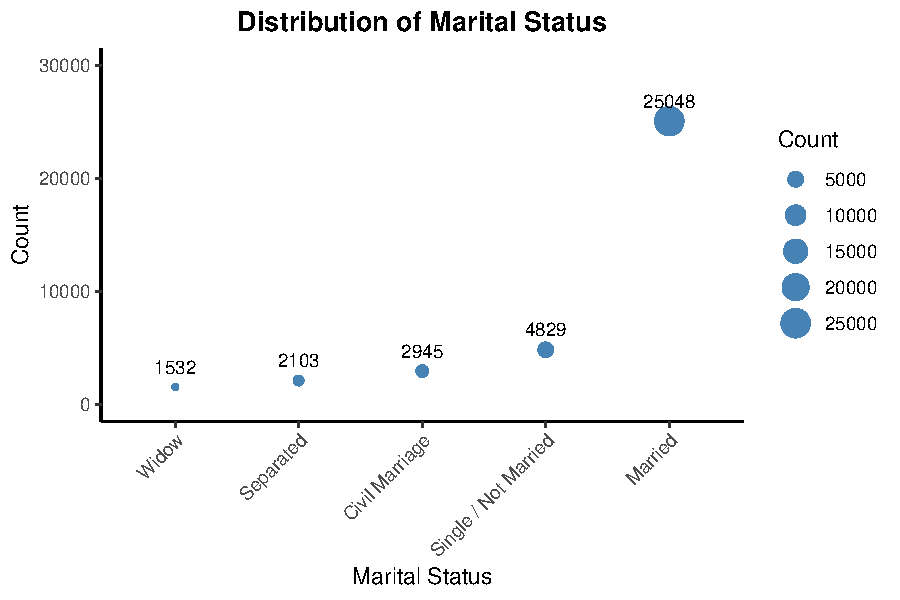
\includegraphics[width=\maxwidth]{figure/unnamed-chunk-21-1} 
\end{knitrout}
\vspace{-10pt} % Reducing space
\caption{Distribution of Marital Status of Customers}
\end{figure}

\begin{knitrout}
\definecolor{shadecolor}{rgb}{0.969, 0.969, 0.969}\color{fgcolor}\begin{kframe}
\begin{alltt}
\hlkwd{analyze_character_column}\hldef{(df,} \hlsng{"Marital.status"}\hldef{)}
\end{alltt}
\begin{verbatim}
## Column: Marital.status 
## Number of unique values: 5 
## Value counts:
##               Category Count Percentage
## 1              Married 25048      68.71
## 2 Single / Not Married  4829      13.25
## 3       Civil Marriage  2945       8.08
## 4            Separated  2103       5.77
## 5                Widow  1532       4.20
\end{verbatim}
\end{kframe}
\end{knitrout}

More three-fifths of customers are married. The next largest group are those who are not married, followed by those who are separated or widowed.

\begin{figure}[H] % [H] ensures figure is placed exactly here
\centering
\begin{knitrout}
\definecolor{shadecolor}{rgb}{0.969, 0.969, 0.969}\color{fgcolor}\begin{kframe}
\begin{alltt}
\hlcom{#install.packages("treemap")}
\hlkwd{library}\hldef{(ggplot2)}
\hlkwd{library}\hldef{(treemap)}

\hldef{dwelling} \hlkwb{<-} \hlkwd{table}\hldef{(df}\hlopt{$}\hldef{Dwelling)}
\hldef{dwelling_df} \hlkwb{<-} \hlkwd{as.data.frame}\hldef{(dwelling)}
\hlkwd{names}\hldef{(dwelling_df)} \hlkwb{<-} \hlkwd{c}\hldef{(}\hlsng{"Dwelling"}\hldef{,} \hlsng{"Count"}\hldef{)}
\hlkwd{treemap}\hldef{(dwelling_df,}
        \hlkwc{index} \hldef{=} \hlsng{"Dwelling"}\hldef{,}
        \hlkwc{vSize} \hldef{=} \hlsng{"Count"}\hldef{,}
        \hlkwc{title} \hldef{=} \hlsng{"Distribution of Dwelling"}\hldef{,}
        \hlkwc{palette} \hldef{=} \hlsng{"Set2"}\hldef{)}
\end{alltt}
\end{kframe}
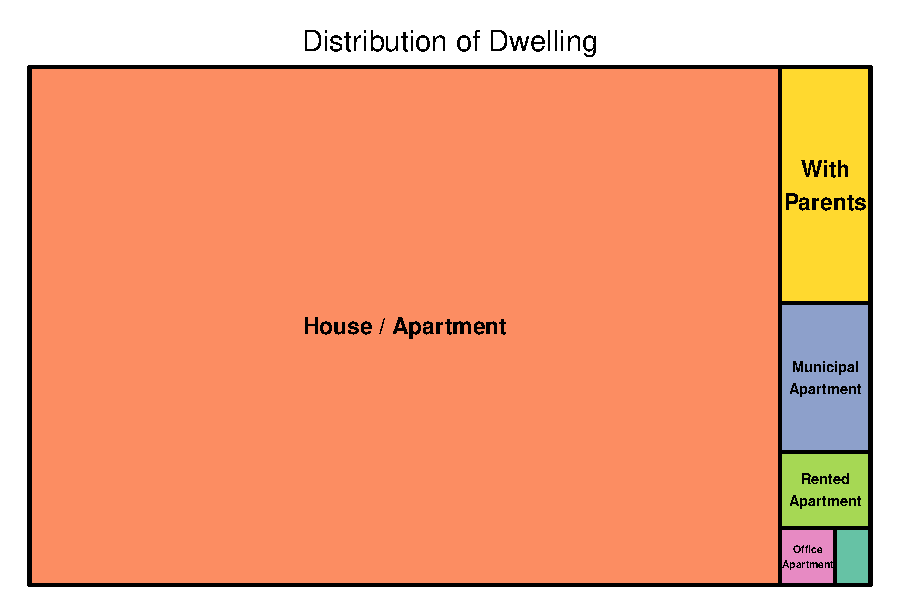
\includegraphics[width=\maxwidth]{figure/unnamed-chunk-23-1} 
\end{knitrout}
\vspace{-10pt} % Reducing space
\caption{Distribution of Customer Dwelling}
\end{figure}

\begin{knitrout}
\definecolor{shadecolor}{rgb}{0.969, 0.969, 0.969}\color{fgcolor}\begin{kframe}
\begin{alltt}
\hlkwd{analyze_character_column}\hldef{(df,} \hlsng{"Dwelling"}\hldef{)}
\end{alltt}
\begin{verbatim}
## Column: Dwelling 
## Number of unique values: 6 
## Value counts:
##              Category Count Percentage
## 1   House / Apartment 32548      89.28
## 2        With Parents  1776       4.87
## 3 Municipal Apartment  1128       3.09
## 4    Rented Apartment   575       1.58
## 5    Office Apartment   262       0.72
## 6     Co-Op Apartment   168       0.46
\end{verbatim}
\end{kframe}
\end{knitrout}

The majority of customers live in a home or apartment, and they make up more than 89\% of the dataset. The rest of the dwellings (a small minority) consist of living with parents, municipal apartments, rented apartments, office apartments, and co-op apartments.

\begin{figure}[H] % [H] ensures figure is placed exactly here
\centering
\begin{knitrout}
\definecolor{shadecolor}{rgb}{0.969, 0.969, 0.969}\color{fgcolor}\begin{kframe}
\begin{alltt}
\hlcom{#install.packages("treemap")}
\hlkwd{library}\hldef{(ggplot2)}
\hlkwd{library}\hldef{(treemap)}

\hldef{job_title} \hlkwb{<-} \hlkwd{table}\hldef{(df}\hlopt{$}\hldef{Job.title)}
\hldef{job_title_df} \hlkwb{<-} \hlkwd{as.data.frame}\hldef{(job_title)}
\hlkwd{names}\hldef{(job_title_df)} \hlkwb{<-} \hlkwd{c}\hldef{(}\hlsng{"Job.title"}\hldef{,} \hlsng{"Count"}\hldef{)}
\hlkwd{treemap}\hldef{(job_title_df,}
        \hlkwc{index} \hldef{=} \hlsng{"Job.title"}\hldef{,}
        \hlkwc{vSize} \hldef{=} \hlsng{"Count"}\hldef{,}
        \hlkwc{title} \hldef{=} \hlsng{"Distribution of Job.title"}\hldef{,}
        \hlkwc{palette} \hldef{=} \hlsng{"Set2"}\hldef{)}
\end{alltt}
\end{kframe}
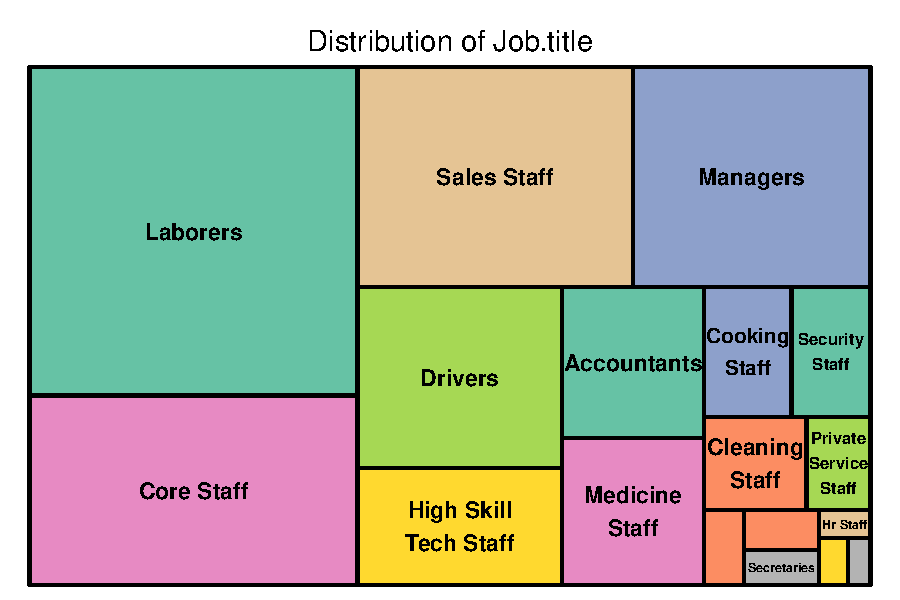
\includegraphics[width=\maxwidth]{figure/unnamed-chunk-25-1} 
\end{knitrout}
\vspace{-10pt} % Reducing space
\caption{Distribution of Customer Dwelling}
\end{figure}

\begin{knitrout}
\definecolor{shadecolor}{rgb}{0.969, 0.969, 0.969}\color{fgcolor}\begin{kframe}
\begin{alltt}
\hlkwd{analyze_character_column}\hldef{(df,} \hlsng{"Job.title"}\hldef{)}
\end{alltt}
\begin{verbatim}
## Column: Job.title 
## Number of unique values: 18 
## Value counts:
##                 Category Count Percentage
## 1               Laborers  6211      24.71
## 2             Core Staff  3591      14.29
## 3            Sales Staff  3485      13.87
## 4               Managers  3012      11.98
## 5                Drivers  2138       8.51
## 6  High Skill Tech Staff  1383       5.50
## 7            Accountants  1241       4.94
## 8         Medicine Staff  1207       4.80
## 9          Cooking Staff   655       2.61
## 10        Security Staff   592       2.36
## 11        Cleaning Staff   551       2.19
## 12 Private Service Staff   344       1.37
## 13    Low-Skill Laborers   175       0.70
## 14  Waiters/Barmen Staff   174       0.69
## 15           Secretaries   151       0.60
## 16              Hr Staff    85       0.34
## 17         Realty Agents    79       0.31
## 18              It Staff    60       0.24
\end{verbatim}
\end{kframe}
\end{knitrout}

`Laborers', `Core Staff' and `Sales Staff' are the most common customer jobs, collectively representing over half of the dataset. `Managers', `Drivers', and `High Skill Tech Staff' also contribute significantly to the job distribution.


\subsubsection{Binary Features}

\begin{knitrout}
\definecolor{shadecolor}{rgb}{0.969, 0.969, 0.969}\color{fgcolor}\begin{kframe}
\begin{alltt}
\hldef{logical_columns} \hlkwb{<-} \hldef{df} \hlopt \hlkwd{select_if}\hldef{(is.logical)}
\hlkwd{names}\hldef{(logical_columns)}
\end{alltt}
\begin{verbatim}
## [1] "Has.a.car"        "Has.a.property"   "Has.a.work.phone" "Has.a.phone"     
## [5] "Has.an.email"     "Is.high.risk"
\end{verbatim}
\end{kframe}
\end{knitrout}

Above are the logical columns explored in this section.

\begin{figure}[H] % [H] ensures figure is placed exactly here
\centering
\begin{knitrout}
\definecolor{shadecolor}{rgb}{0.969, 0.969, 0.969}\color{fgcolor}\begin{kframe}
\begin{alltt}
\hldef{plot_df} \hlkwb{<-} \hlkwd{data.frame}\hldef{(}
  \hlkwc{col_name} \hldef{=} \hlkwd{c}\hldef{(}\hlsng{"Has.a.car"}\hldef{,}
               \hlsng{"Has.a.property"}\hldef{,} \hlsng{"Has.a.work.phone"}\hldef{,}
               \hlsng{"Has.a.phone"}\hldef{,} \hlsng{"Has.an.email"}\hldef{),}
  \hlkwc{true} \hldef{=} \hlkwd{c}\hldef{(}\hlkwd{sum}\hldef{(df}\hlopt{$}\hldef{Has.a.car),}
           \hlkwd{sum}\hldef{(df}\hlopt{$}\hldef{Has.a.property),} \hlkwd{sum}\hldef{(df}\hlopt{$}\hldef{Has.a.work.phone),}
           \hlkwd{sum}\hldef{(df}\hlopt{$}\hldef{Has.a.phone),} \hlkwd{sum}\hldef{(df}\hlopt{$}\hldef{Has.an.email)),}
  \hlkwc{false} \hldef{=} \hlkwd{c}\hldef{(}\hlkwd{nrow}\hldef{(df)} \hlopt{-} \hlkwd{sum}\hldef{(df}\hlopt{$}\hldef{Has.a.car),}
            \hlkwd{nrow}\hldef{(df)} \hlopt{-} \hlkwd{sum}\hldef{(df}\hlopt{$}\hldef{Has.a.property),} \hlkwd{nrow}\hldef{(df)} \hlopt{-} \hlkwd{sum}\hldef{(df}\hlopt{$}\hldef{Has.a.work.phone),}
            \hlkwd{nrow}\hldef{(df)} \hlopt{-} \hlkwd{sum}\hldef{(df}\hlopt{$}\hldef{Has.a.phone),} \hlkwd{nrow}\hldef{(df)} \hlopt{-} \hlkwd{sum}\hldef{(df}\hlopt{$}\hldef{Has.an.email))}
\hldef{)}

\hldef{plot_df_long} \hlkwb{<-} \hldef{tidyr}\hlopt{::}\hlkwd{pivot_longer}\hldef{(plot_df,} \hlkwc{cols} \hldef{=} \hlkwd{c}\hldef{(}\hlsng{"true"}\hldef{,} \hlsng{"false"}\hldef{),}
                                    \hlkwc{names_to} \hldef{=} \hlsng{"value"}\hldef{,} \hlkwc{values_to} \hldef{=} \hlsng{"count"}\hldef{)}

\hlkwd{ggplot}\hldef{(plot_df_long,} \hlkwd{aes}\hldef{(}\hlkwc{x} \hldef{= col_name,} \hlkwc{y} \hldef{= count} \hlopt{/} \hlkwd{nrow}\hldef{(df)} \hlopt{*} \hlnum{100}\hldef{,} \hlkwc{fill} \hldef{= value))} \hlopt{+}
  \hlkwd{geom_bar}\hldef{(}\hlkwc{stat} \hldef{=} \hlsng{"identity"}\hldef{)} \hlopt{+}
  \hlkwd{labs}\hldef{(}\hlkwc{x} \hldef{=} \hlsng{"Binary Features"}\hldef{,} \hlkwc{y} \hldef{=} \hlsng{"Percentage"}\hldef{,} \hlkwc{fill} \hldef{=} \hlkwa{NULL}\hldef{)} \hlopt{+}
  \hlkwd{geom_text}\hldef{(}\hlkwd{aes}\hldef{(}\hlkwc{label} \hldef{= count),} \hlkwc{position} \hldef{=} \hlkwd{position_stack}\hldef{(}\hlkwc{vjust} \hldef{=} \hlnum{0.5}\hldef{),} \hlkwc{size} \hldef{=} \hlnum{3}\hldef{)} \hlopt{+}
  \hlkwd{theme_bw}\hldef{()} \hlopt{+}
  \hlkwd{theme}\hldef{(}\hlkwc{legend.position} \hldef{=} \hlsng{"bottom"}\hldef{)}
\end{alltt}
\end{kframe}
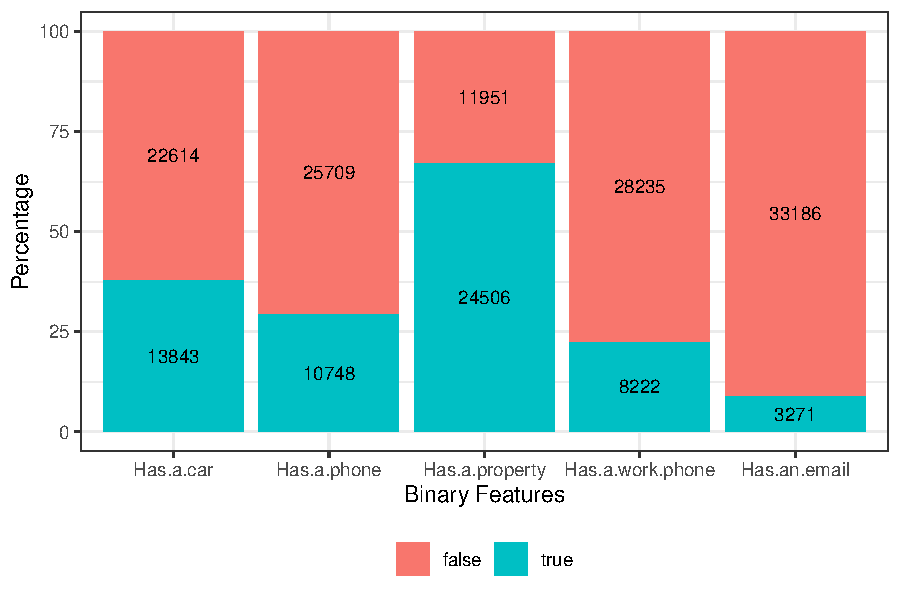
\includegraphics[width=\maxwidth]{figure/unnamed-chunk-28-1} 
\end{knitrout}
\caption{Distribution of Five Binary Features}
\end{figure}

More than three-fifths of the customer do not have cars. Customer with cars make up a smaller but still significant group within the dataset. \\

There are significantly more customers who owns property as compared with those who do not. \\

Surprisingly, most customers do not have neither a work phone nor a personal phone. This could mean customer did not include their phone contact details during creation of their accounts. \\

Only around 9\% of the customers provided their email address. Rest of the customers either did not provide it or do not have an email.  \\

\begin{figure}[H] % [H] ensures figure is placed exactly here
\centering
\begin{knitrout}
\definecolor{shadecolor}{rgb}{0.969, 0.969, 0.969}\color{fgcolor}\begin{kframe}
\begin{alltt}
\hlcom{#install.packages("lessR")}
\hlkwd{library}\hldef{(lessR)}

\hlkwd{PieChart}\hldef{(Is.high.risk,} \hlkwc{data} \hldef{= df,}
         \hlkwc{hole} \hldef{=} \hlnum{0.4}\hldef{,}
         \hlkwc{fill} \hldef{=} \hlsng{'blues'}\hldef{,}
         \hlkwc{color} \hldef{=} \hlsng{"black"}\hldef{,}
         \hlkwc{lwd} \hldef{=} \hlnum{1.5}\hldef{,}
         \hlkwc{main} \hldef{=} \hlsng{"Distribution of Is.high.risk"}\hldef{)}
\end{alltt}
\end{kframe}
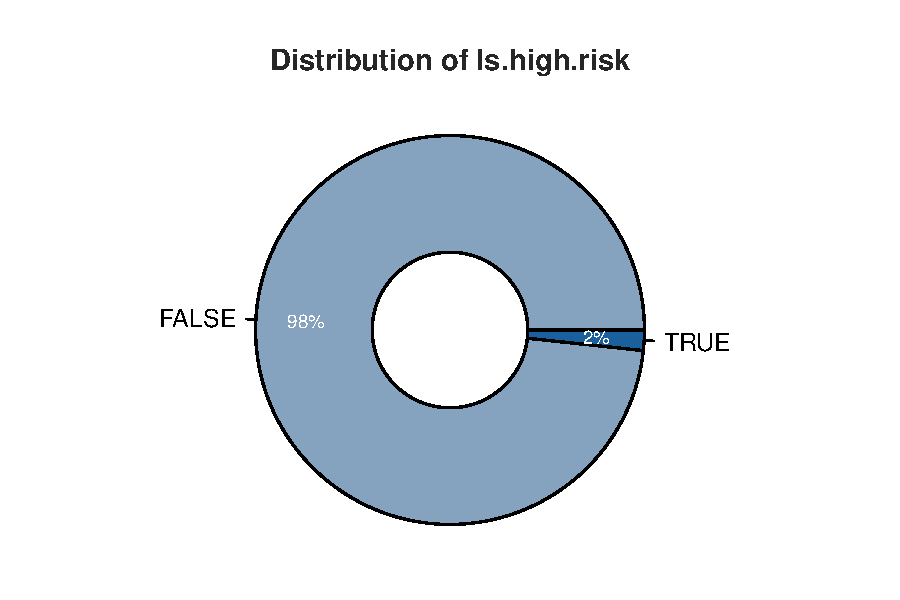
\includegraphics[width=\maxwidth]{figure/unnamed-chunk-29-1} 
\end{knitrout}
\vspace{-10pt} % Reducing space
\caption{Distribution of Customer Risk}
\end{figure}

Almost all customers are classified as low risk in the dataset. High Risk customer makes up around 1.69\% in the dataset.  \\

\subsubsection{Numerical Features}

\begin{knitrout}
\definecolor{shadecolor}{rgb}{0.969, 0.969, 0.969}\color{fgcolor}\begin{kframe}
\begin{alltt}
\hldef{numeric_columns} \hlkwb{<-} \hldef{df} \hlopt \hlkwd{select_if}\hldef{(}\hlkwa{function}\hldef{(}\hlkwc{x}\hldef{)} \hlkwd{is.integer}\hldef{(x)} \hlopt{||} \hlkwd{is.numeric}\hldef{(x))}
\hlkwd{names}\hldef{(numeric_columns)}
\end{alltt}
\begin{verbatim}
## [1] "Children.count"             "Income"                    
## [3] "Customer.relative.age"      "Employment.relative.length"
## [5] "Family.member.count"        "Account.relative.age"
\end{verbatim}
\end{kframe}
\end{knitrout}

Above features are explored in this section. The three columns: `Customer.relative.age', `Employment.relative.length', and `Account.relative.age' are measured by subtracting the actual value from a reference point value. So, they can contain negative values.     


\begin{figure}[H] % [H] ensures figure is placed exactly here
\centering
\begin{knitrout}
\definecolor{shadecolor}{rgb}{0.969, 0.969, 0.969}\color{fgcolor}\begin{kframe}
\begin{alltt}
\hlkwd{ggplot}\hldef{(df,} \hlkwd{aes_string}\hldef{(}\hlkwc{x} \hldef{=} \hlsng{"Children.count"}\hldef{))} \hlopt{+}
  \hlkwd{geom_bar}\hldef{(}\hlkwd{aes}\hldef{(}\hlkwc{fill} \hldef{=} \hlkwd{cut}\hldef{(Children.count,} \hlkwc{breaks} \hldef{=} \hlkwd{c}\hldef{(}\hlopt{-}\hlnum{Inf}\hldef{,} \hlnum{0}\hldef{,} \hlnum{1}\hldef{,} \hlnum{2}\hldef{,} \hlnum{3}\hldef{,} \hlnum{4}\hldef{,} \hlnum{5}\hldef{,} \hlnum{Inf}\hldef{))),}
           \hlkwc{show.legend} \hldef{=} \hlnum{FALSE}\hldef{)} \hlopt{+}
  \hlkwd{geom_text}\hldef{(}\hlkwc{stat} \hldef{=} \hlsng{"count"}\hldef{,} \hlkwd{aes}\hldef{(}\hlkwc{label} \hldef{= ..count..),} \hlkwc{vjust} \hldef{=} \hlopt{-}\hlnum{0.5}\hldef{,} \hlkwc{size}\hldef{=}\hlnum{3}\hldef{)} \hlopt{+}
  \hlkwd{labs}\hldef{(}\hlkwc{title} \hldef{=} \hlkwd{paste0}\hldef{(}\hlsng{"Distribution of Children.count"}\hldef{),}
       \hlkwc{x} \hldef{=} \hlsng{"Number of Children"}\hldef{,}
       \hlkwc{y} \hldef{=} \hlsng{"Count"}\hldef{)} \hlopt{+}
  \hlkwd{theme_classic}\hldef{()}\hlopt{+}
  \hlkwd{theme}\hldef{(}\hlkwc{plot.title} \hldef{=} \hlkwd{element_text}\hldef{(}\hlkwc{hjust} \hldef{=} \hlnum{0.5}\hldef{,} \hlkwc{face} \hldef{=} \hlsng{"bold"}\hldef{))} \hlopt{+}
  \hlkwd{scale_x_continuous}\hldef{(}\hlkwc{limits} \hldef{=} \hlkwd{c}\hldef{(}\hlopt{-}\hlnum{1}\hldef{,} \hlnum{6}\hldef{),} \hlkwc{breaks} \hldef{=} \hlkwd{seq}\hldef{(}\hlnum{0}\hldef{,} \hlnum{5}\hldef{,} \hlkwc{by} \hldef{=} \hlnum{1}\hldef{))} \hlopt{+}
  \hlkwd{scale_fill_brewer}\hldef{(}\hlkwc{palette} \hldef{=} \hlsng{"Set2"}\hldef{)}
\end{alltt}
\end{kframe}
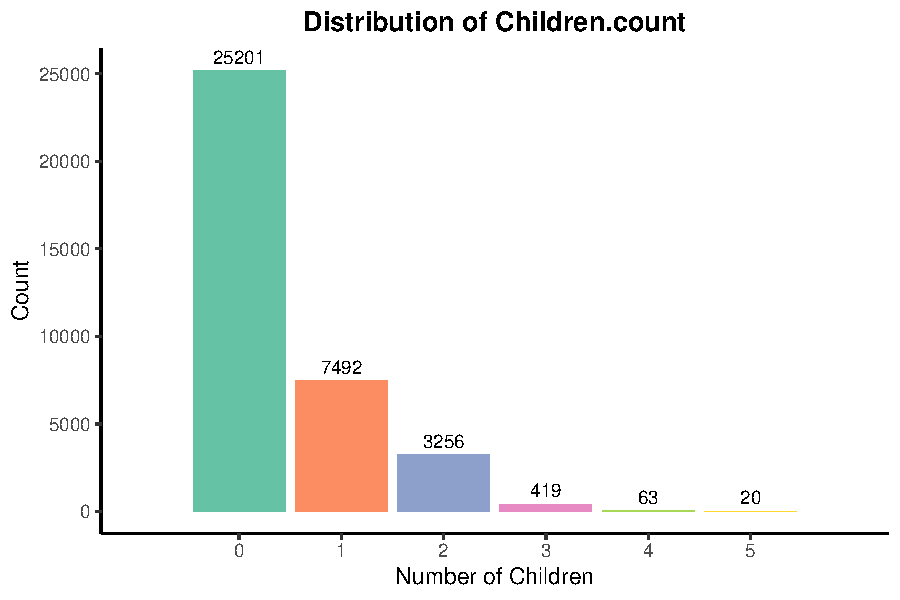
\includegraphics[width=\maxwidth]{figure/unnamed-chunk-31-1} 
\end{knitrout}
\vspace{0pt} % Reducing space
\caption{Distribution of Childred Customers Have}
\end{figure}

\begin{knitrout}
\definecolor{shadecolor}{rgb}{0.969, 0.969, 0.969}\color{fgcolor}\begin{kframe}
\begin{alltt}
\hlkwd{table}\hldef{(df}\hlopt{$}\hldef{Children.count)}
\end{alltt}
\begin{verbatim}
## 
##     0     1     2     3     4     5     7    14    19 
## 25201  7492  3256   419    63    20     2     3     1
\end{verbatim}
\end{kframe}
\end{knitrout}

Most customers have no children. There is a single customer with highest number of children of 19. Majority of the customers have either no children, 1 child or 2 children. \\

\begin{figure}[H] % [H] ensures figure is placed exactly here
\centering
\begin{knitrout}
\definecolor{shadecolor}{rgb}{0.969, 0.969, 0.969}\color{fgcolor}\begin{kframe}
\begin{alltt}
\hlkwd{ggplot}\hldef{(df,} \hlkwd{aes_string}\hldef{(}\hlkwc{x} \hldef{=} \hlsng{"Family.member.count"}\hldef{))} \hlopt{+}
  \hlkwd{geom_bar}\hldef{(}
    \hlkwd{aes}\hldef{(}\hlkwc{fill} \hldef{=} \hlkwd{cut}\hldef{(Family.member.count,} \hlkwc{breaks} \hldef{=} \hlkwd{c}\hldef{(}\hlopt{-}\hlnum{Inf}\hldef{,} \hlnum{1}\hldef{,} \hlnum{2}\hldef{,} \hlnum{3}\hldef{,} \hlnum{4}\hldef{,} \hlnum{5}\hldef{,} \hlnum{6}\hldef{,} \hlnum{7}\hldef{,} \hlnum{Inf}\hldef{))),}
    \hlkwc{show.legend} \hldef{=} \hlnum{FALSE}\hldef{)} \hlopt{+}
  \hlkwd{geom_text}\hldef{(}\hlkwc{stat} \hldef{=} \hlsng{"count"}\hldef{,} \hlkwd{aes}\hldef{(}\hlkwc{label} \hldef{= ..count..),} \hlkwc{vjust} \hldef{=} \hlopt{-}\hlnum{0.5}\hldef{,} \hlkwc{size} \hldef{=} \hlnum{3}\hldef{)} \hlopt{+}
  \hlkwd{labs}\hldef{(}\hlkwc{title} \hldef{=} \hlkwd{paste0}\hldef{(}\hlsng{"Distribution of Family.member.count"}\hldef{),}
       \hlkwc{x} \hldef{=} \hlsng{"Number of Family Members"}\hldef{,}
       \hlkwc{y} \hldef{=} \hlsng{"Count"}\hldef{)} \hlopt{+}
  \hlkwd{theme_classic}\hldef{()} \hlopt{+}
  \hlkwd{theme}\hldef{(}\hlkwc{plot.title} \hldef{=} \hlkwd{element_text}\hldef{(}\hlkwc{hjust} \hldef{=} \hlnum{0.5}\hldef{,} \hlkwc{face} \hldef{=} \hlsng{"bold"}\hldef{))} \hlopt{+}
  \hlkwd{scale_x_continuous}\hldef{(}\hlkwc{limits} \hldef{=} \hlkwd{c}\hldef{(}\hlnum{0}\hldef{,} \hlnum{8}\hldef{),} \hlkwc{breaks} \hldef{=} \hlkwd{seq}\hldef{(}\hlnum{1}\hldef{,} \hlnum{7}\hldef{,} \hlkwc{by} \hldef{=} \hlnum{1}\hldef{))} \hlopt{+}
  \hlkwd{scale_fill_brewer}\hldef{(}\hlkwc{palette} \hldef{=} \hlsng{"Set2"}\hldef{)}
\end{alltt}
\end{kframe}
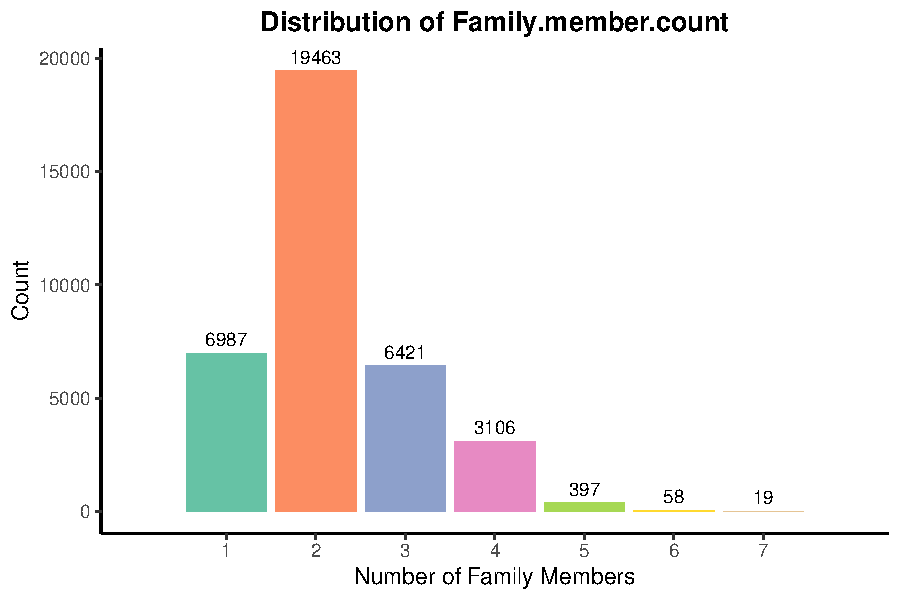
\includegraphics[width=\maxwidth]{figure/unnamed-chunk-33-1} 
\end{knitrout}
\vspace{0pt} % Reducing space
\caption{Distribution of Number of Customer Family Members}
\end{figure}

The majority of customers report having 2 family members, followed by those reporting 1 or 3 family members with nearly equal proportions between the two categories. \\

\begin{figure}[H] % [H] ensures figure is placed exactly here
\centering
\begin{knitrout}
\definecolor{shadecolor}{rgb}{0.969, 0.969, 0.969}\color{fgcolor}\begin{kframe}
\begin{alltt}
\hlkwd{ggplot}\hldef{(df,} \hlkwd{aes_string}\hldef{(}\hlkwc{x} \hldef{=} \hlsng{"Customer.relative.age"}\hldef{))} \hlopt{+}
  \hlkwd{geom_histogram}\hldef{(}\hlkwd{aes}\hldef{(}\hlkwc{fill} \hldef{= ..count..),} \hlkwc{bins} \hldef{=} \hlnum{60}\hldef{,} \hlkwc{show.legend} \hldef{=} \hlnum{FALSE}\hldef{)} \hlopt{+}
  \hlkwd{labs}\hldef{(}\hlkwc{title} \hldef{=} \hlkwd{paste0}\hldef{(}\hlsng{"Distribution of Customer.relative.age"}\hldef{),}
       \hlkwc{x} \hldef{=} \hlsng{"Relative Age"}\hldef{,}
       \hlkwc{y} \hldef{=} \hlsng{"Count"}\hldef{)} \hlopt{+}
  \hlkwd{theme_classic}\hldef{()} \hlopt{+}
  \hlkwd{theme}\hldef{(}\hlkwc{plot.title} \hldef{=} \hlkwd{element_text}\hldef{(}\hlkwc{hjust} \hldef{=} \hlnum{0.5}\hldef{,} \hlkwc{face} \hldef{=} \hlsng{"bold"}\hldef{),}
        \hlkwc{panel.grid.major.y} \hldef{=} \hlkwd{element_line}\hldef{(}\hlkwc{linetype} \hldef{=} \hlsng{"dashed"}\hldef{,} \hlkwc{color} \hldef{=} \hlsng{"gray"}\hldef{))} \hlopt{+}
  \hlkwd{scale_y_continuous}\hldef{(}\hlkwc{limits} \hldef{=} \hlkwd{c}\hldef{(}\hlnum{0}\hldef{,} \hlnum{1000}\hldef{))} \hlopt{+}
  \hlkwd{scale_fill_gradient}\hldef{(}\hlkwc{low} \hldef{=} \hlsng{"#132c45"}\hldef{,} \hlkwc{high} \hldef{=} \hlsng{"#54a7e7"}\hldef{)}
\end{alltt}
\end{kframe}
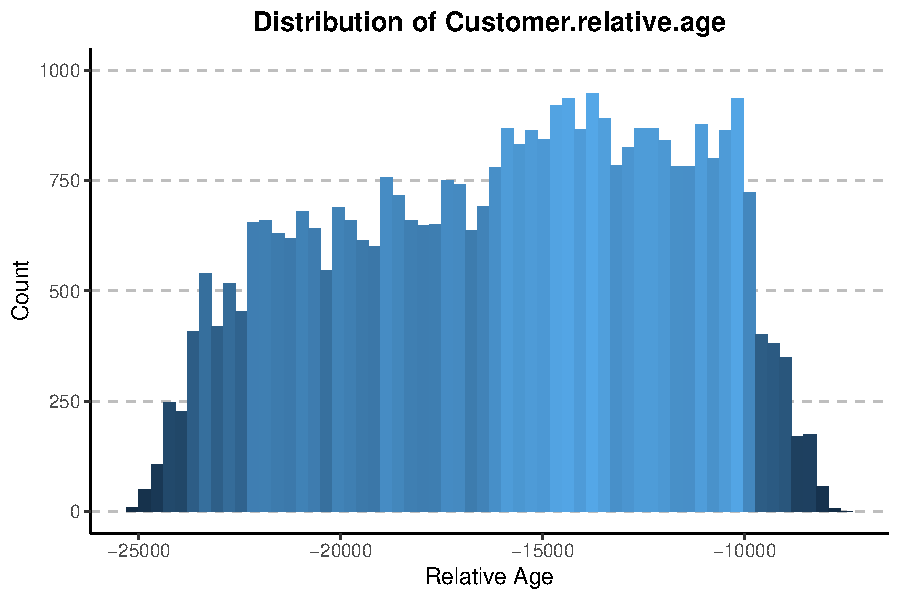
\includegraphics[width=\maxwidth]{figure/unnamed-chunk-34-1} 
\end{knitrout}
\vspace{0pt} % Reducing space
\caption{Distribution of Relative Age of Customers}
\end{figure}

When comparing the ages of customers, a higher proportion falls into the younger age group. \\

\begin{figure}[H] % [H] ensures figure is placed exactly here
\centering
\begin{knitrout}
\definecolor{shadecolor}{rgb}{0.969, 0.969, 0.969}\color{fgcolor}\begin{kframe}
\begin{alltt}
\hlkwd{ggplot}\hldef{(df,} \hlkwd{aes_string}\hldef{(}\hlkwc{x} \hldef{=} \hlsng{"Account.relative.age"}\hldef{))} \hlopt{+}
  \hlkwd{geom_histogram}\hldef{(}\hlkwd{aes}\hldef{(}\hlkwc{fill} \hldef{= ..count..),} \hlkwc{bins} \hldef{=} \hlnum{30}\hldef{,} \hlkwc{show.legend} \hldef{=} \hlnum{FALSE}\hldef{)} \hlopt{+}
  \hlkwd{labs}\hldef{(}\hlkwc{title} \hldef{=} \hlkwd{paste0}\hldef{(}\hlsng{"Distribution of Account.relative.age"}\hldef{),}
       \hlkwc{x} \hldef{=} \hlsng{"Relative Account Age"}\hldef{,}
       \hlkwc{y} \hldef{=} \hlsng{"Count"}\hldef{)} \hlopt{+}
  \hlkwd{theme_classic}\hldef{()} \hlopt{+}
  \hlkwd{theme}\hldef{(}\hlkwc{plot.title} \hldef{=} \hlkwd{element_text}\hldef{(}\hlkwc{hjust} \hldef{=} \hlnum{0.5}\hldef{,} \hlkwc{face} \hldef{=} \hlsng{"bold"}\hldef{),}
        \hlkwc{panel.grid.major.y} \hldef{=} \hlkwd{element_line}\hldef{(}\hlkwc{linetype} \hldef{=} \hlsng{"dashed"}\hldef{,} \hlkwc{color} \hldef{=} \hlsng{"gray"}\hldef{))} \hlopt{+}
  \hlkwd{scale_y_continuous}\hldef{(}\hlkwc{limits} \hldef{=} \hlkwd{c}\hldef{(}\hlnum{0}\hldef{,} \hlnum{2000}\hldef{))} \hlopt{+}
  \hlkwd{scale_fill_gradient}\hldef{(}\hlkwc{low} \hldef{=} \hlsng{"#132c45"}\hldef{,} \hlkwc{high} \hldef{=} \hlsng{"#54a7e7"}\hldef{)}
\end{alltt}
\end{kframe}
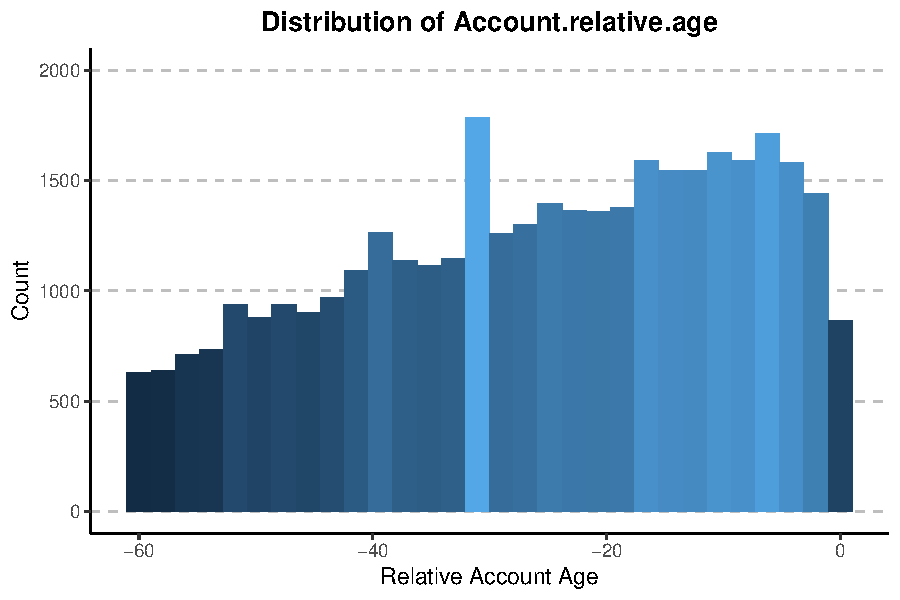
\includegraphics[width=\maxwidth]{figure/unnamed-chunk-35-1} 
\end{knitrout}
\vspace{0pt} % Reducing space
\caption{Distribution of Relative Age of Cutomer's Account}
\end{figure}

Similar trend is observed in the distribution of relative age of accounts where comparatively more proportion of accounts seem to created recently. \\


\begin{knitrout}
\definecolor{shadecolor}{rgb}{0.969, 0.969, 0.969}\color{fgcolor}\begin{kframe}
\begin{alltt}
\hlcom{#install.packages('patchwork')}
\hlkwd{library}\hldef{(patchwork)}
\hlkwd{library}\hldef{(ggplot2)}

\hldef{df_neg} \hlkwb{<-} \hldef{df[df}\hlopt{$}\hldef{Employment.relative.length} \hlopt{<=} \hlnum{0}\hldef{, ]}
\hldef{df_pos} \hlkwb{<-} \hldef{df[df}\hlopt{$}\hldef{Employment.relative.length} \hlopt{>} \hlnum{0}\hldef{, ]}

\hldef{bins} \hlkwb{<-} \hlnum{30}

\hldef{p1} \hlkwb{<-} \hlkwd{ggplot}\hldef{(df_neg,} \hlkwd{aes}\hldef{(}\hlkwc{x} \hldef{= Employment.relative.length))} \hlopt{+}
  \hlkwd{geom_histogram}\hldef{(}\hlkwd{aes}\hldef{(}\hlkwc{fill} \hldef{= ..count..),} \hlkwc{bins} \hldef{= bins,} \hlkwc{show.legend} \hldef{=} \hlnum{FALSE}\hldef{)} \hlopt{+}
  \hlkwd{labs}\hldef{(}\hlkwc{title} \hldef{=} \hlsng{"Employment Period"}\hldef{,}
       \hlkwc{x} \hldef{=} \hlsng{"Relative Duration"}\hldef{,}
       \hlkwc{y} \hldef{=} \hlsng{"Count"}\hldef{)} \hlopt{+}
  \hlkwd{theme_classic}\hldef{()} \hlopt{+}
  \hlkwd{theme}\hldef{(}
    \hlkwc{plot.title} \hldef{=} \hlkwd{element_text}\hldef{(}\hlkwc{hjust} \hldef{=} \hlnum{0.5}\hldef{,} \hlkwc{face} \hldef{=} \hlsng{"bold"}\hldef{),}
    \hlkwc{panel.grid.major.y} \hldef{=} \hlkwd{element_line}\hldef{(}\hlkwc{linetype} \hldef{=} \hlsng{"dashed"}\hldef{,} \hlkwc{color} \hldef{=} \hlsng{"gray"}\hldef{))} \hlopt{+}
  \hlkwd{scale_y_continuous}\hldef{(}\hlkwc{limits} \hldef{=} \hlkwd{c}\hldef{(}\hlnum{0}\hldef{,} \hlnum{6500}\hldef{))} \hlopt{+}
  \hlkwd{scale_fill_gradient}\hldef{(}\hlkwc{low} \hldef{=} \hlsng{"#132c45"}\hldef{,} \hlkwc{high} \hldef{=} \hlsng{"#54a7e7"}\hldef{)}

\hldef{p2_start} \hlkwb{=} \hlnum{360000}
\hldef{p2} \hlkwb{<-} \hlkwd{ggplot}\hldef{(df_pos,} \hlkwd{aes}\hldef{(}\hlkwc{x} \hldef{= Employment.relative.length))} \hlopt{+}
  \hlkwd{geom_histogram}\hldef{(}\hlkwd{aes}\hldef{(}\hlkwc{fill} \hldef{= ..count..),} \hlkwc{bins} \hldef{= bins,} \hlkwc{show.legend} \hldef{=} \hlnum{FALSE}\hldef{)} \hlopt{+}
  \hlkwd{labs}\hldef{(}\hlkwc{title} \hldef{=} \hlsng{"Unemployment Period"}\hldef{,}
       \hlkwc{x} \hldef{=} \hlsng{"Relative Duration"}\hldef{,}
       \hlkwc{y} \hldef{=} \hlsng{"Count"}\hldef{)} \hlopt{+}
  \hlkwd{theme_classic}\hldef{()} \hlopt{+}
  \hlkwd{theme}\hldef{(}
    \hlkwc{plot.title} \hldef{=} \hlkwd{element_text}\hldef{(}\hlkwc{hjust} \hldef{=} \hlnum{0.5}\hldef{,} \hlkwc{face} \hldef{=} \hlsng{"bold"}\hldef{),}
    \hlkwc{panel.grid.major.y} \hldef{=} \hlkwd{element_line}\hldef{(}\hlkwc{linetype} \hldef{=} \hlsng{"dashed"}\hldef{,} \hlkwc{color} \hldef{=} \hlsng{"gray"}\hldef{))}  \hlopt{+}
  \hlkwd{scale_x_continuous}\hldef{(}\hlkwc{limits} \hldef{=} \hlkwd{c}\hldef{(p2_start, p2_start} \hlopt{+} \hlnum{15000}\hldef{))} \hlopt{+}
  \hlkwd{scale_y_continuous}\hldef{(}\hlkwc{limits} \hldef{=} \hlkwd{c}\hldef{(}\hlnum{0}\hldef{,} \hlnum{6500}\hldef{))} \hlopt{+}
  \hlkwd{scale_fill_gradient}\hldef{(}\hlkwc{low} \hldef{=} \hlsng{"#132c45"}\hldef{,} \hlkwc{high} \hldef{=} \hlsng{"#54a7e7"}\hldef{)}

\hldef{p1} \hlopt{+} \hldef{p2}
\end{alltt}
\end{kframe}\begin{figure}[H]
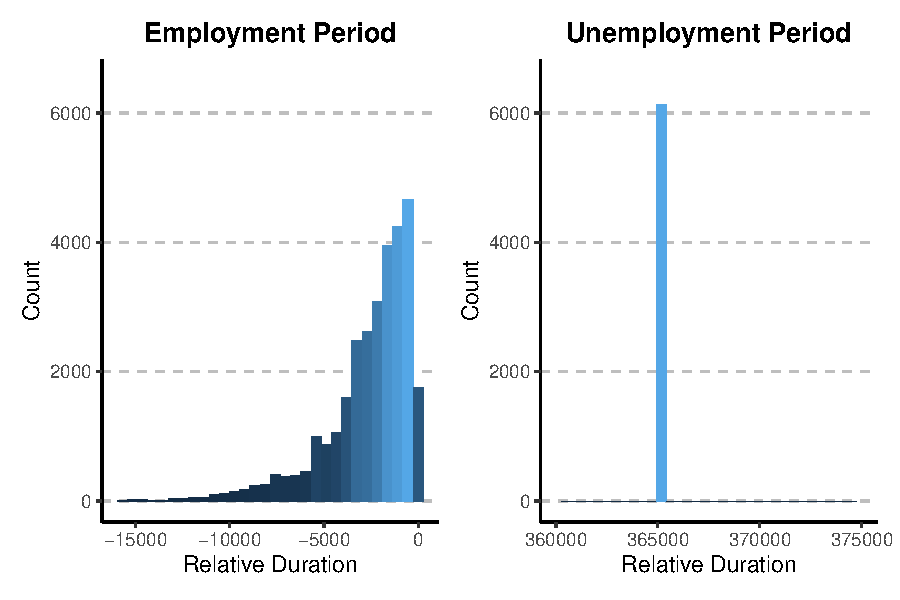
\includegraphics[width=\maxwidth]{figure/unnamed-chunk-36-1} \caption[Distribution of Relative Employment Length]{Distribution of Relative Employment Length}\label{fig:unnamed-chunk-36}
\end{figure}

\end{knitrout}

In the `Employment.relative.length' column, negative values mean employment periods. Significantly higher proportion of customers are employed. \\


\begin{figure}[H] % [H] ensures figure is placed exactly here
\centering
\begin{knitrout}
\definecolor{shadecolor}{rgb}{0.969, 0.969, 0.969}\color{fgcolor}\begin{kframe}
\begin{alltt}
\hlkwd{ggplot}\hldef{(df,} \hlkwd{aes_string}\hldef{(}\hlkwc{x} \hldef{=} \hlsng{"Income"}\hldef{))} \hlopt{+}
  \hlkwd{geom_histogram}\hldef{(}\hlkwd{aes}\hldef{(}\hlkwc{fill} \hldef{= ..count..),} \hlkwc{bins} \hldef{=} \hlnum{60}\hldef{,} \hlkwc{show.legend} \hldef{=} \hlnum{FALSE}\hldef{)} \hlopt{+}
  \hlkwd{labs}\hldef{(}\hlkwc{title} \hldef{=} \hlkwd{paste0}\hldef{(}\hlsng{"Distribution of Income"}\hldef{),}
       \hlkwc{x} \hldef{=} \hlsng{"Income"}\hldef{,}
       \hlkwc{y} \hldef{=} \hlsng{"Count"}\hldef{)} \hlopt{+}
  \hlkwd{theme_classic}\hldef{()} \hlopt{+}
  \hlkwd{theme}\hldef{(}\hlkwc{plot.title} \hldef{=} \hlkwd{element_text}\hldef{(}\hlkwc{hjust} \hldef{=} \hlnum{0.5}\hldef{,} \hlkwc{face} \hldef{=} \hlsng{"bold"}\hldef{),}
        \hlkwc{panel.background} \hldef{=} \hlkwd{element_blank}\hldef{(),}
        \hlkwc{panel.grid.major.y} \hldef{=} \hlkwd{element_line}\hldef{(}\hlkwc{linetype} \hldef{=} \hlsng{"dashed"}\hldef{,} \hlkwc{color} \hldef{=} \hlsng{"gray"}\hldef{))}  \hlopt{+}
  \hlkwd{scale_x_continuous}\hldef{(}\hlkwc{labels} \hldef{=} \hlkwa{function}\hldef{(}\hlkwc{x}\hldef{)} \hlkwd{format}\hldef{(x,} \hlkwc{scientific} \hldef{=} \hlnum{FALSE}\hldef{))} \hlopt{+}
  \hlkwd{scale_fill_gradient}\hldef{(}\hlkwc{low} \hldef{=} \hlsng{"#132c45"}\hldef{,} \hlkwc{high} \hldef{=} \hlsng{"#54a7e7"}\hldef{)}
\end{alltt}
\end{kframe}
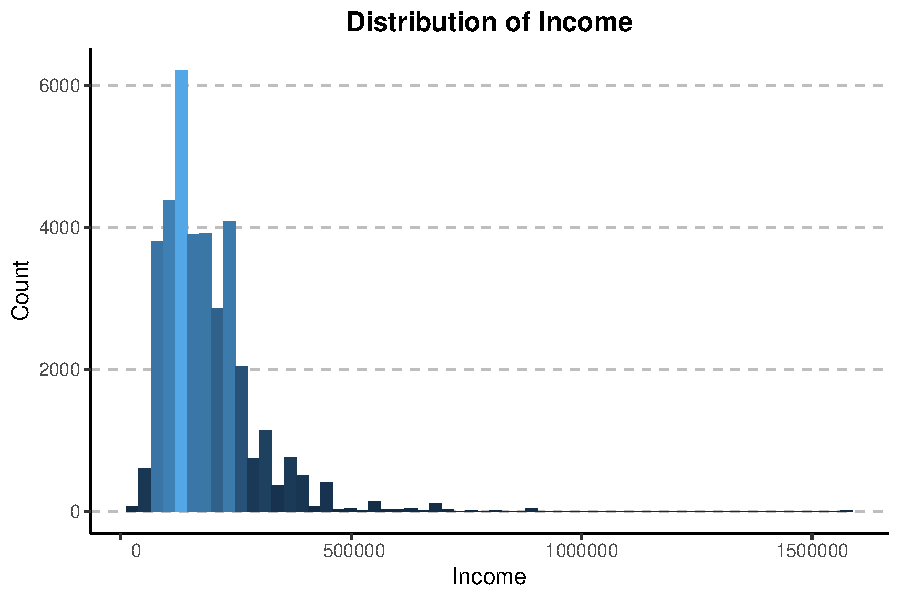
\includegraphics[width=\maxwidth]{figure/unnamed-chunk-37-1} 
\end{knitrout}
\vspace{0pt} % Reducing space
\caption{Distribution of Income of Customers}
\end{figure}






















\newpage
\section{Experimental Results}

The experimental results to the previously stated non-trivial research questions were obtained using multivariate analysis and predictive modeling. It required grouping, pivoting or transforming data which were then analyzed conducted using high quality graphs made using ggplot2.\\

\subsection{What factors greatly contribute to risk status of customers for credit card?}

The approach to obtaining solution in this section includes creating a XGBoost classifer model and visualizing its feature importance. The target feature is `Is.high.risk'.\\

\begin{knitrout}
\definecolor{shadecolor}{rgb}{0.969, 0.969, 0.969}\color{fgcolor}\begin{kframe}
\begin{alltt}
\hlcom{# install.packages("reshape2")}
\hlcom{# install.packages("ggplot2")}
\hlkwd{library}\hldef{(reshape2)}
\hlkwd{library}\hldef{(ggplot2)}

\hldef{numeric_cols} \hlkwb{<-} \hlkwd{sapply}\hldef{(}
  \hldef{df,} \hlkwa{function}\hldef{(}\hlkwc{x}\hldef{)} \hlkwd{is.numeric}\hldef{(x)} \hlopt{|} \hlkwd{is.integer}\hldef{(x)} \hlopt{|} \hlkwd{is.logical}\hldef{(x)}
\hldef{)}
\hldef{df_numeric} \hlkwb{<-} \hldef{df[, numeric_cols]}
\hldef{cormat} \hlkwb{<-} \hlkwd{round}\hldef{(}\hlkwd{cor}\hldef{(df_numeric),}\hlnum{2}\hldef{)}

\hldef{upper_tri} \hlkwb{<-} \hldef{cormat}
\hldef{upper_tri[}\hlkwd{lower.tri}\hldef{(cormat)]} \hlkwb{<-} \hlnum{NA}

\hldef{melted_cormat} \hlkwb{<-} \hlkwd{melt}\hldef{(upper_tri,} \hlkwc{na.rm} \hldef{=} \hlnum{TRUE}\hldef{)}

\hlkwd{ggplot}\hldef{(}\hlkwc{data} \hldef{= melted_cormat,} \hlkwd{aes}\hldef{(Var2, Var1,} \hlkwc{fill} \hldef{= value))}\hlopt{+}
  \hlkwd{geom_tile}\hldef{(}\hlkwc{color} \hldef{=} \hlsng{"white"}\hldef{)}\hlopt{+}
  \hlkwd{scale_fill_gradient2}\hldef{(}\hlkwc{low} \hldef{=} \hlsng{"blue"}\hldef{,} \hlkwc{high} \hldef{=} \hlsng{"red"}\hldef{,} \hlkwc{mid} \hldef{=} \hlsng{"white"}\hldef{,}
                       \hlkwc{midpoint} \hldef{=} \hlnum{0}\hldef{,} \hlkwc{limit} \hldef{=} \hlkwd{c}\hldef{(}\hlopt{-}\hlnum{1}\hldef{,}\hlnum{1}\hldef{),} \hlkwc{space} \hldef{=} \hlsng{"Lab"}\hldef{,}
                       \hlkwc{name}\hldef{=}\hlsng{"Pearson\textbackslash{}nCorrelation"}\hldef{)} \hlopt{+}
  \hlkwd{theme_minimal}\hldef{()}\hlopt{+}
  \hlkwd{theme}\hldef{(}\hlkwc{axis.text.x} \hldef{=} \hlkwd{element_text}\hldef{(}\hlkwc{angle} \hldef{=} \hlnum{45}\hldef{,} \hlkwc{vjust} \hldef{=} \hlnum{1}\hldef{,}
                                   \hlkwc{size} \hldef{=} \hlnum{12}\hldef{,} \hlkwc{hjust} \hldef{=} \hlnum{1}\hldef{))}\hlopt{+}
  \hlkwd{coord_fixed}\hldef{()} \hlopt{+}
  \hlkwd{geom_text}\hldef{(}\hlkwd{aes}\hldef{(Var2, Var1,} \hlkwc{label} \hldef{= value),} \hlkwc{color} \hldef{=} \hlsng{"black"}\hldef{,} \hlkwc{size} \hldef{=} \hlnum{4}\hldef{)} \hlopt{+}
  \hlkwd{theme}\hldef{(}
    \hlkwc{axis.title.x} \hldef{=} \hlkwd{element_blank}\hldef{(),}
    \hlkwc{axis.title.y} \hldef{=} \hlkwd{element_blank}\hldef{(),}
    \hlkwc{panel.grid.major} \hldef{=} \hlkwd{element_blank}\hldef{(),}
    \hlkwc{panel.border} \hldef{=} \hlkwd{element_blank}\hldef{(),}
    \hlkwc{panel.background} \hldef{=} \hlkwd{element_blank}\hldef{(),}
    \hlkwc{axis.ticks} \hldef{=} \hlkwd{element_blank}\hldef{(),}
    \hlkwc{legend.justification} \hldef{=} \hlkwd{c}\hldef{(}\hlnum{1}\hldef{,} \hlnum{0}\hldef{),}
    \hlkwc{legend.position} \hldef{=} \hlkwd{c}\hldef{(}\hlnum{0.6}\hldef{,} \hlnum{0.7}\hldef{),}
    \hlkwc{legend.direction} \hldef{=} \hlsng{"horizontal"}\hldef{)}\hlopt{+}
  \hlkwd{guides}\hldef{(}\hlkwc{fill} \hldef{=} \hlkwd{guide_colorbar}\hldef{(}\hlkwc{barwidth} \hldef{=} \hlnum{7}\hldef{,} \hlkwc{barheight} \hldef{=} \hlnum{1}\hldef{,}
                               \hlkwc{title.position} \hldef{=} \hlsng{"top"}\hldef{,} \hlkwc{title.hjust} \hldef{=} \hlnum{0.5}\hldef{))}
\end{alltt}
\end{kframe}\begin{figure}[H]
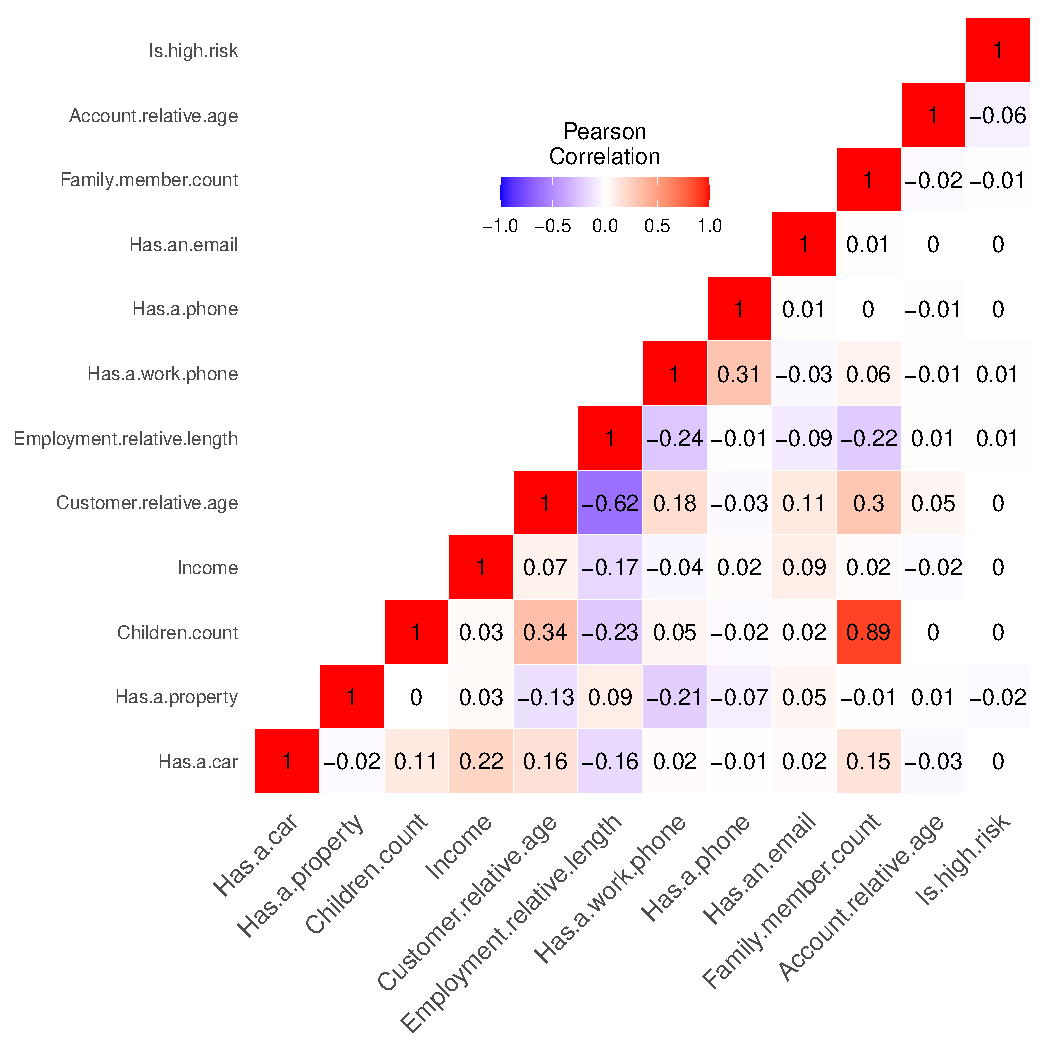
\includegraphics[width=\maxwidth]{figure/unnamed-chunk-38-1} \caption[Correlation Heatmap]{Correlation Heatmap}\label{fig:unnamed-chunk-38}
\end{figure}

\end{knitrout}

No features seem to be correlated with the target feature `Is.high.risk'.\\

\begin{knitrout}
\definecolor{shadecolor}{rgb}{0.969, 0.969, 0.969}\color{fgcolor}\begin{kframe}
\begin{alltt}
\hlcom{# install.packages("xgboost")}
\hlcom{# install.packages("SHAPforxgboost")}
\hlcom{# install.packages("caret")}
\hlkwd{library}\hldef{(xgboost)}
\hlkwd{library}\hldef{(SHAPforxgboost)}
\hlkwd{library}\hldef{(caret)}
\end{alltt}
\end{kframe}
\end{knitrout}

Above necessary libraries were imported.\\

\begin{knitrout}
\definecolor{shadecolor}{rgb}{0.969, 0.969, 0.969}\color{fgcolor}\begin{kframe}
\begin{alltt}
\hldef{df_clean} \hlkwb{<-} \hlkwd{na.omit}\hldef{(df)}

\hldef{features} \hlkwb{<-} \hldef{df_clean[,} \hlopt{!}\hldef{(}\hlkwd{names}\hldef{(df_clean)} \hlopt \hlkwd{c}\hldef{(}\hlsng{"Is.high.risk"}\hldef{))]} \hlcom{# Exclude target column}
\hldef{target} \hlkwb{<-} \hldef{df_clean}\hlopt{$}\hldef{Is.high.risk}

\hlcom{# Train-Test Split}

\hlkwd{set.seed}\hldef{(}\hlnum{555}\hldef{)} \hlcom{# for reproducibility}
\hldef{train_size} \hlkwb{<-} \hlkwd{floor}\hldef{(}\hlnum{0.8} \hlopt{*} \hlkwd{nrow}\hldef{(features))}
\hldef{train_indices} \hlkwb{<-} \hlkwd{sample}\hldef{(}\hlkwd{seq_len}\hldef{(}\hlkwd{nrow}\hldef{(features)),} \hlkwc{size} \hldef{= train_size)}

\hldef{X_train} \hlkwb{<-} \hldef{features[train_indices, ]}
\hldef{preprocessed_data} \hlkwb{<-} \hlkwd{dummyVars}\hldef{(}\hlsng{" ~ ."}\hldef{,} \hlkwc{data} \hldef{= X_train)}
\hldef{X_train} \hlkwb{<-} \hlkwd{data.frame}\hldef{(}\hlkwd{predict}\hldef{(preprocessed_data,} \hlkwc{newdata} \hldef{= X_train))}
\hldef{X_train} \hlkwb{=} \hlkwd{as.matrix}\hldef{(X_train)}

\hldef{y_train} \hlkwb{<-} \hldef{target[train_indices]}
\hldef{y_train} \hlkwb{<-} \hlkwd{as.numeric}\hldef{(y_train)}

\hldef{X_test} \hlkwb{<-} \hldef{features[}\hlopt{-}\hldef{train_indices, ]}
\hldef{preprocessed_data} \hlkwb{<-} \hlkwd{dummyVars}\hldef{(}\hlsng{" ~ ."}\hldef{,} \hlkwc{data} \hldef{= X_test)}
\hldef{X_test} \hlkwb{<-} \hlkwd{data.frame}\hldef{(}\hlkwd{predict}\hldef{(preprocessed_data,} \hlkwc{newdata} \hldef{= X_test))}
\hldef{X_test} \hlkwb{=} \hlkwd{as.matrix}\hldef{(X_test)}

\hldef{y_test} \hlkwb{<-} \hldef{target[}\hlopt{-}\hldef{train_indices]}
\hldef{y_test} \hlkwb{<-} \hlkwd{as.numeric}\hldef{(y_test)}

\hlkwd{dim}\hldef{(X_train)}
\end{alltt}
\begin{verbatim}
## [1] 20107    57
\end{verbatim}
\begin{alltt}
\hlkwd{dim}\hldef{(X_test)}
\end{alltt}
\begin{verbatim}
## [1] 5027   57
\end{verbatim}
\end{kframe}
\end{knitrout}

The wrangled dataframe was split into train-test split of 0.8 and then one-hot-encoded. 80\% was used for training and 20\% for testing . \\

\begin{knitrout}
\definecolor{shadecolor}{rgb}{0.969, 0.969, 0.969}\color{fgcolor}\begin{kframe}
\begin{alltt}
\hldef{dtrain} \hlkwb{<-} \hlkwd{xgb.DMatrix}\hldef{(}\hlkwc{data} \hldef{= X_train,} \hlkwc{label}\hldef{=y_train)}
\hldef{dtest} \hlkwb{<-} \hlkwd{xgb.DMatrix}\hldef{(}\hlkwc{data} \hldef{= X_test,} \hlkwc{label}\hldef{=y_test)}
\hldef{watchlist} \hlkwb{<-} \hlkwd{list}\hldef{(}\hlkwc{train}\hldef{=dtrain,} \hlkwc{test}\hldef{=dtest)}
\end{alltt}
\end{kframe}
\end{knitrout}

The train-test splits were converted to DMatrix objects which are used to efficiently store the data in a format optimized for training and evaluating an XGBoost model. \\

\begin{knitrout}
\definecolor{shadecolor}{rgb}{0.969, 0.969, 0.969}\color{fgcolor}\begin{kframe}
\begin{alltt}
\hldef{model} \hlkwb{<-} \hlkwd{xgb.train}\hldef{(}
  \hlkwc{data}\hldef{=dtrain,}
  \hlkwc{lambda} \hldef{=} \hlnum{5}\hldef{,}
  \hlkwc{alpha}\hldef{=}\hlnum{5}\hldef{,}
  \hlkwc{max.depth}\hldef{=}\hlnum{4}\hldef{,}
  \hlkwc{eta}\hldef{=}\hlnum{0.3}\hldef{,}
  \hlkwc{subsample}\hldef{=}\hlnum{0.8}\hldef{,}
  \hlkwc{colsample_bytree}\hldef{=}\hlnum{0.9}\hldef{,}
  \hlkwc{nthread} \hldef{=} \hlnum{3}\hldef{,}
  \hlkwc{nrounds}\hldef{=}\hlnum{1000}\hldef{,}
  \hlkwc{scale_pos_weight} \hldef{=} \hlnum{30}\hldef{,}
  \hlkwc{watchlist}\hldef{=watchlist,}
  \hlkwc{objective} \hldef{=} \hlsng{"binary:logistic"}\hldef{,}
  \hlkwc{eval_metric} \hldef{=} \hlsng{"logloss"}\hldef{,}
  \hlkwc{verbose} \hldef{=} \hlnum{0}
\hldef{)}

\hldef{y_pred} \hlkwb{=} \hlkwd{predict}\hldef{(model, X_test)}
\hldef{y_pred} \hlkwb{<-} \hlkwd{ifelse}\hldef{(y_pred} \hlopt{>} \hlnum{0.5}\hldef{,} \hlnum{1}\hldef{,} \hlnum{0}\hldef{)}
\hldef{y_test_factor} \hlkwb{<-} \hlkwd{factor}\hldef{(y_test,} \hlkwc{levels} \hldef{=} \hlkwd{c}\hldef{(}\hlnum{0}\hldef{,} \hlnum{1}\hldef{))}
\hldef{y_pred_factor} \hlkwb{<-} \hlkwd{factor}\hldef{(y_pred,} \hlkwc{levels} \hldef{=} \hlkwd{c}\hldef{(}\hlnum{0}\hldef{,} \hlnum{1}\hldef{))}
\hlkwd{confusionMatrix}\hldef{(y_test_factor, y_pred_factor)}
\end{alltt}
\begin{verbatim}
## Confusion Matrix and Statistics
## 
##           Reference
## Prediction    0    1
##          0 4888   62
##          1   47   30
##                                           
##                Accuracy : 0.9783          
##                  95% CI : (0.9739, 0.9822)
##     No Information Rate : 0.9817          
##     P-Value [Acc > NIR] : 0.9644          
##                                           
##                   Kappa : 0.3441          
##                                           
##  Mcnemar's Test P-Value : 0.1799          
##                                           
##             Sensitivity : 0.9905          
##             Specificity : 0.3261          
##          Pos Pred Value : 0.9875          
##          Neg Pred Value : 0.3896          
##              Prevalence : 0.9817          
##          Detection Rate : 0.9723          
##    Detection Prevalence : 0.9847          
##       Balanced Accuracy : 0.6583          
##                                           
##        'Positive' Class : 0               
## 
\end{verbatim}
\end{kframe}
\end{knitrout}

The hyperparameters of the model was set manually through trial and error resulting in a model that has an accuracy of almost 98\% and a high number of true negatives (4888) but relatively fewer true positives (30) in test dataset. \\

\begin{knitrout}
\definecolor{shadecolor}{rgb}{0.969, 0.969, 0.969}\color{fgcolor}\begin{kframe}
\begin{alltt}
\hlcom{# install.packages("Ckmeans.1d.dp")}
\hlkwd{library}\hldef{(Ckmeans.1d.dp)}
\hldef{importance_matrix} \hlkwb{<-} \hlkwd{xgb.importance}\hldef{(}\hlkwd{colnames}\hldef{(X_train),} \hlkwc{model} \hldef{= model)}
\hldef{xgb.ggplt} \hlkwb{<-} \hlkwd{xgb.ggplot.importance}\hldef{(}
  \hlkwc{importance_matrix} \hldef{= importance_matrix,} \hlkwc{top_n} \hldef{=} \hlnum{5}
\hldef{)}
\hldef{xgb.ggplt} \hlopt{+}
  \hlkwd{theme_classic}\hldef{()} \hlopt{+}
  \hlkwd{theme}\hldef{(}\hlkwc{legend.position} \hldef{=} \hlsng{"bottom"}\hldef{)} \hlopt{+}
  \hlkwd{labs}\hldef{(}\hlkwc{title} \hldef{=} \hlsng{"Important Features for Classifying Credit Card Risk"}\hldef{,}
       \hlkwc{y} \hldef{=} \hlsng{"Feature Importance Score (XGBoost)"}\hldef{)} \hlopt{+}
  \hlkwd{theme}\hldef{(}\hlkwc{plot.title} \hldef{=} \hlkwd{element_text}\hldef{(}\hlkwc{face} \hldef{=} \hlsng{"bold"}\hldef{))}
\end{alltt}
\end{kframe}\begin{figure}[H]
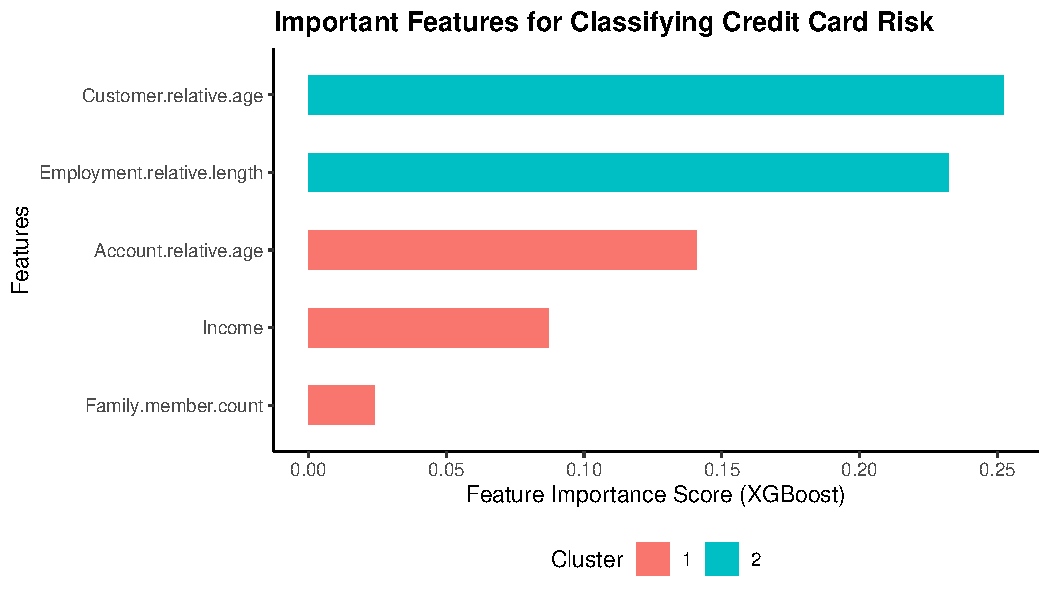
\includegraphics[width=\maxwidth]{figure/unnamed-chunk-43-1} \caption[Top Five Important Features for Classifying Customer Risk]{Top Five Important Features for Classifying Customer Risk}\label{fig:unnamed-chunk-43}
\end{figure}

\end{knitrout}

\subsubsection{Analysis and answer}

Employment tenure and customer age demonstrated the strongest impact on risk status, followed by account age. How much a customer earn, and to a lesser extent how many family members they have, also contributes. This suggests that stability and longevity in personal and financial aspects are more predictive of credit card risk. Given all these points, financial stability and longevity in personal and financial aspects are key predictors of credit card risk, with employment length and customer age exhibiting the most pronounced influence when classifying customers into high risk or low risk.\\


\subsection{Which professions have a higher chance of being classified as high risk?}

\begin{knitrout}
\definecolor{shadecolor}{rgb}{0.969, 0.969, 0.969}\color{fgcolor}\begin{kframe}
\begin{alltt}
\hlkwd{library}\hldef{(ggplot2)}

\hldef{job_counts} \hlkwb{<-} \hlkwd{table}\hldef{(df}\hlopt{$}\hldef{Job.title, df}\hlopt{$}\hldef{Is.high.risk)}
\hldef{job_counts_df} \hlkwb{<-} \hlkwd{as.data.frame}\hldef{(job_counts)}
\hldef{job_counts_df} \hlkwb{<-} \hldef{job_counts_df} \hlopt \hlkwd{pivot_wider}\hldef{(}
  \hlkwc{names_from} \hldef{= Var2,} \hlkwc{values_from} \hldef{= Freq}
\hldef{)}

\hlkwd{colnames}\hldef{(job_counts_df)} \hlkwb{<-} \hlkwd{c}\hldef{(}\hlsng{"Job.title"}\hldef{,} \hlsng{"Low.risk"}\hldef{,} \hlsng{"High.risk"}\hldef{)}

\hldef{job_counts_df} \hlkwb{<-} \hldef{job_counts_df} \hlopt
  \hlkwd{mutate}\hldef{(}
    \hlkwc{Low.risk.perct} \hldef{=} \hlkwd{round}\hldef{((Low.risk} \hlopt{/} \hldef{(Low.risk} \hlopt{+} \hldef{High.risk))} \hlopt{*} \hlnum{100}\hldef{,} \hlnum{3}\hldef{),}
    \hlkwc{High.risk.perct} \hldef{=} \hlkwd{round}\hldef{((High.risk} \hlopt{/} \hldef{(Low.risk} \hlopt{+} \hldef{High.risk))} \hlopt{*} \hlnum{100}\hldef{,} \hlnum{3}\hldef{)}
  \hldef{)}

\hldef{job_counts_df} \hlkwb{<-} \hldef{job_counts_df} \hlopt
  \hlkwd{arrange}\hldef{(}\hlkwd{desc}\hldef{(High.risk.perct))}


\hldef{job_counts_df} \hlkwb{<-} \hldef{job_counts_df} \hlopt
  \hlkwd{mutate}\hldef{(}\hlkwc{Risk} \hldef{=} \hlkwd{case_when}\hldef{(}
    \hldef{High.risk.perct} \hlopt{>} \hlnum{4} \hlopt{~} \hlsng{"Very High Risk"}\hldef{,}
    \hldef{High.risk.perct} \hlopt{<} \hlnum{1} \hlopt{~} \hlsng{"Low Risk"}\hldef{,}
    \hlnum{TRUE} \hlopt{~} \hlsng{"Moderate Risk"}
  \hldef{))}

\hldef{risk_colors} \hlkwb{<-} \hlkwd{c}\hldef{(}
  \hlsng{"Very High Risk"} \hldef{=} \hlsng{"#f3661f"}\hldef{,}
  \hlsng{"Low Risk"} \hldef{=} \hlsng{"#50bb6d"}\hldef{,}
  \hlsng{"Moderate Risk"} \hldef{=} \hlsng{"#1470bb"}
\hldef{)}

\hlkwd{ggplot}\hldef{(}
  \hldef{job_counts_df,}
  \hlkwd{aes}\hldef{(}\hlkwc{x} \hldef{= High.risk.perct,} \hlkwc{y} \hldef{=} \hlkwd{reorder}\hldef{(Job.title, High.risk.perct),} \hlkwc{fill} \hldef{= Risk)}
  \hldef{)} \hlopt{+}
  \hlkwd{geom_bar}\hldef{(}\hlkwc{stat} \hldef{=} \hlsng{"identity"}\hldef{,} \hlkwc{width} \hldef{=} \hlnum{0.7}\hldef{,} \hlkwc{color} \hldef{=} \hlnum{NA}\hldef{)} \hlopt{+}
  \hlkwd{geom_text}\hldef{(}\hlkwd{aes}\hldef{(}\hlkwc{label} \hldef{=} \hlkwd{paste0}\hldef{(}\hlkwd{round}\hldef{(High.risk.perct,} \hlnum{1}\hldef{),} \hlsng{"%"}\hldef{)),}
            \hlkwc{hjust} \hldef{=} \hlopt{-}\hlnum{0.5}\hldef{,}
            \hlkwc{vjust} \hldef{=} \hlnum{0.4}\hldef{,}
            \hlkwc{color} \hldef{=} \hlsng{"black"}\hldef{,}
            \hlkwc{size} \hldef{=} \hlnum{3}\hldef{)} \hlopt{+}
  \hlkwd{geom_vline}\hldef{(}\hlkwc{xintercept} \hldef{=} \hlnum{0}\hldef{,} \hlkwc{color} \hldef{=} \hlsng{"black"}\hldef{,} \hlkwc{linetype} \hldef{=} \hlsng{"solid"}\hldef{)} \hlopt{+}
  \hlkwd{scale_fill_identity}\hldef{(}
    \hlkwc{name} \hldef{=} \hlsng{""}\hldef{,}
    \hlkwc{guide} \hldef{=} \hlkwd{guide_legend}\hldef{(}\hlkwc{title.position} \hldef{=} \hlsng{"top"}\hldef{,} \hlkwc{title.hjust} \hldef{=} \hlnum{0.5}\hldef{))} \hlopt{+}
  \hlkwd{labs}\hldef{(}
    \hlkwc{title} \hldef{=} \hlsng{"Examining High-Risk Job Titles in Credit Card Applications"}\hldef{,}
    \hlkwc{subtitle} \hldef{=} \hlsng{"(Percentage of High Risk Individuals)"}\hldef{,}
  \hldef{)} \hlopt{+}
  \hlkwd{theme_minimal}\hldef{()} \hlopt{+}
  \hlkwd{theme}\hldef{(}
    \hlkwc{plot.title} \hldef{=} \hlkwd{element_text}\hldef{(}\hlkwc{size} \hldef{=} \hlnum{14}\hldef{,} \hlkwc{face} \hldef{=} \hlsng{"bold"}\hldef{,} \hlkwc{hjust} \hldef{=} \hlnum{0}\hldef{),}
    \hlkwc{plot.subtitle} \hldef{=} \hlkwd{element_text}\hldef{(}\hlkwc{size} \hldef{=} \hlnum{12}\hldef{,} \hlkwc{hjust} \hldef{=} \hlnum{0}\hldef{,} \hlkwc{margin} \hldef{=} \hlkwd{margin}\hldef{(}\hlkwc{b} \hldef{=} \hlnum{15}\hldef{)),}
    \hlkwc{panel.grid.major.x} \hldef{=} \hlkwd{element_line}\hldef{(}\hlkwc{linetype} \hldef{=} \hlsng{"dashed"}\hldef{,} \hlkwc{color} \hldef{=} \hlsng{"gray"}\hldef{),}
    \hlkwc{panel.grid.major.y} \hldef{=} \hlkwd{element_blank}\hldef{(),}
    \hlkwc{panel.grid.minor.x} \hldef{=} \hlkwd{element_blank}\hldef{(),}
    \hlkwc{panel.grid.minor.y} \hldef{=} \hlkwd{element_blank}\hldef{(),}
    \hlkwc{axis.text.y} \hldef{=} \hlkwd{element_text}\hldef{(}\hlkwc{size} \hldef{=} \hlnum{10}\hldef{,} \hlkwc{face} \hldef{=} \hlsng{"bold"}\hldef{),}
    \hlkwc{axis.title} \hldef{=} \hlkwd{element_text}\hldef{(}\hlkwc{size} \hldef{=} \hlnum{12}\hldef{),}
    \hlkwc{axis.text.x} \hldef{=} \hlkwd{element_blank}\hldef{(),}
    \hlkwc{axis.title.x} \hldef{=} \hlkwd{element_blank}\hldef{(),}
    \hlkwc{axis.title.y} \hldef{=} \hlkwd{element_blank}\hldef{(),}
    \hlkwc{legend.position} \hldef{=} \hlsng{"bottom"}
  \hldef{)} \hlopt{+}
  \hlkwd{scale_fill_manual}\hldef{(}\hlkwc{values} \hldef{= risk_colors,} \hlkwc{name} \hldef{=} \hlsng{""}\hldef{)}
\end{alltt}
\end{kframe}\begin{figure}[H]
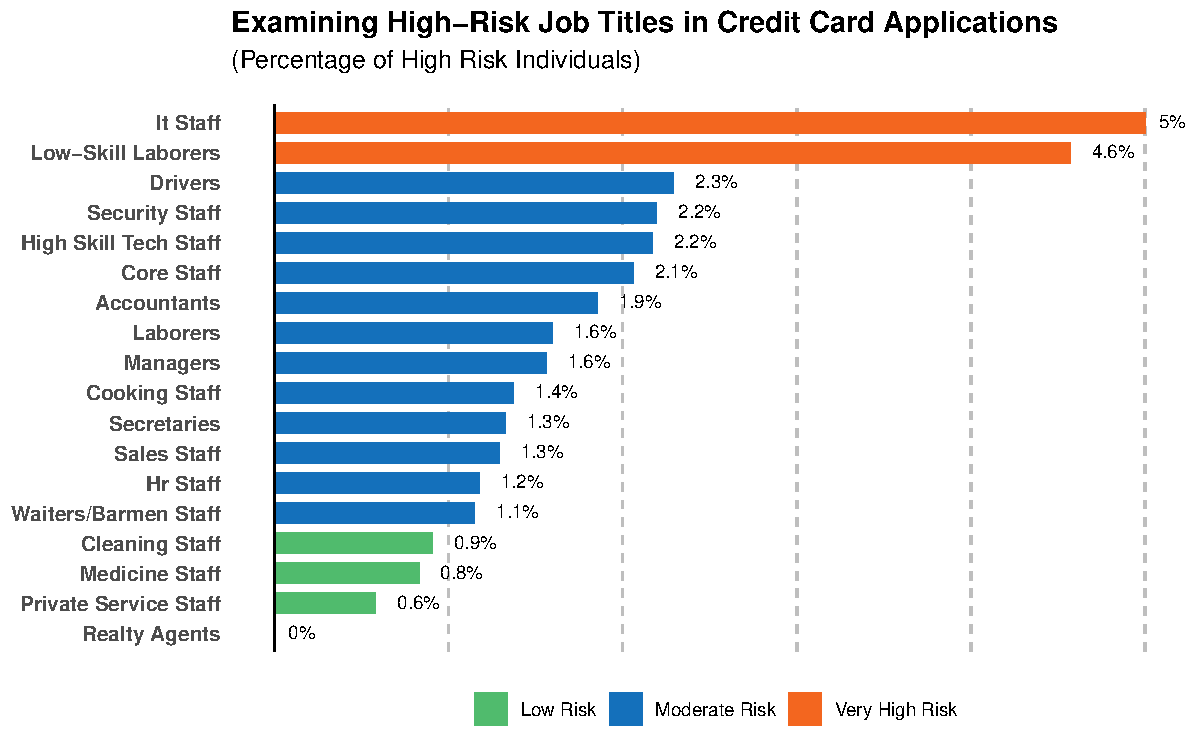
\includegraphics[width=\maxwidth]{figure/unnamed-chunk-44-1} \caption[High-Risk Jobs]{High-Risk Jobs}\label{fig:unnamed-chunk-44}
\end{figure}

\end{knitrout}

\begin{knitrout}
\definecolor{shadecolor}{rgb}{0.969, 0.969, 0.969}\color{fgcolor}\begin{kframe}
\begin{alltt}
\hlcom{#install.packages("ggridges")}
\hlkwd{library}\hldef{(ggridges)}
\hlkwd{library}\hldef{(ggplot2)}

\hldef{df_clean} \hlkwb{<-} \hlkwd{na.omit}\hldef{(df)}

\hldef{df_clean}\hlopt{$}\hldef{Risk} \hlkwb{<-}  \hlkwd{with}\hldef{(}
  \hldef{df_clean,}
  \hlkwd{ifelse}\hldef{(}
    \hldef{Job.title} \hlopt \hlkwd{c}\hldef{(}\hlsng{'It Staff'}\hldef{,} \hlsng{'Low-Skill Laborers'}\hldef{),}
    \hlsng{'Very High Risk'}\hldef{,}
    \hlkwd{ifelse}\hldef{(}
      \hldef{Job.title} \hlopt \hlkwd{c}\hldef{(}
        \hlsng{'Cleaning Staff'}\hldef{,} \hlsng{'Medicine Staff'}\hldef{,}
        \hlsng{'Private Service Staff'}\hldef{,} \hlsng{'Realty Agents'}\hldef{),}
      \hlsng{'Low Risk'}\hldef{,}
      \hlsng{'Moderate Risk'}\hldef{)}
    \hldef{)}
  \hldef{)}

\hldef{risk_colors} \hlkwb{<-} \hlkwd{c}\hldef{(}
  \hlsng{"Very High Risk"} \hldef{=} \hlsng{"#f3661f"}\hldef{,}
  \hlsng{"Low Risk"} \hldef{=} \hlsng{"#50bb6d"}\hldef{,}
  \hlsng{"Moderate Risk"} \hldef{=} \hlsng{"#1470bb"}
\hldef{)}

\hlkwd{ggplot}\hldef{(df_clean,} \hlkwd{aes}\hldef{(}\hlkwc{x} \hldef{= Income,} \hlkwc{y} \hldef{= Job.title,} \hlkwc{fill} \hldef{= Risk))} \hlopt{+}
  \hlkwd{geom_density_ridges}\hldef{()} \hlopt{+}
  \hlkwd{theme_ridges}\hldef{()} \hlopt{+}
  \hlkwd{theme}\hldef{(}\hlkwc{legend.position} \hldef{=} \hlsng{"bottom"}\hldef{)} \hlopt{+}
  \hlkwd{scale_fill_manual}\hldef{(}\hlkwc{values} \hldef{= risk_colors,} \hlkwc{name} \hldef{=} \hlsng{""}\hldef{)} \hlopt{+}
  \hlkwd{theme_ridges}\hldef{()} \hlopt{+}
  \hlkwd{theme}\hldef{(}\hlkwc{legend.position} \hldef{=} \hlsng{"bottom"}\hldef{,}
        \hlkwc{plot.title} \hldef{=} \hlkwd{element_text}\hldef{(}\hlkwc{hjust} \hldef{=} \hlnum{0.5}\hldef{))} \hlopt{+}
  \hlkwd{scale_x_continuous}\hldef{(}\hlkwc{limits} \hldef{=} \hlkwd{c}\hldef{(}\hlopt{-}\hlnum{1}\hldef{,} \hlnum{1000000}\hldef{))} \hlopt{+}
  \hlkwd{labs}\hldef{(}\hlkwc{title} \hldef{=} \hlsng{"Income Distribution by Job Title Risk"}\hldef{,}
       \hlkwc{x} \hldef{=} \hlsng{"Income"}\hldef{,}
       \hlkwc{y} \hldef{=} \hlsng{"Job Title"}\hldef{)}
\end{alltt}
\end{kframe}\begin{figure}[H]
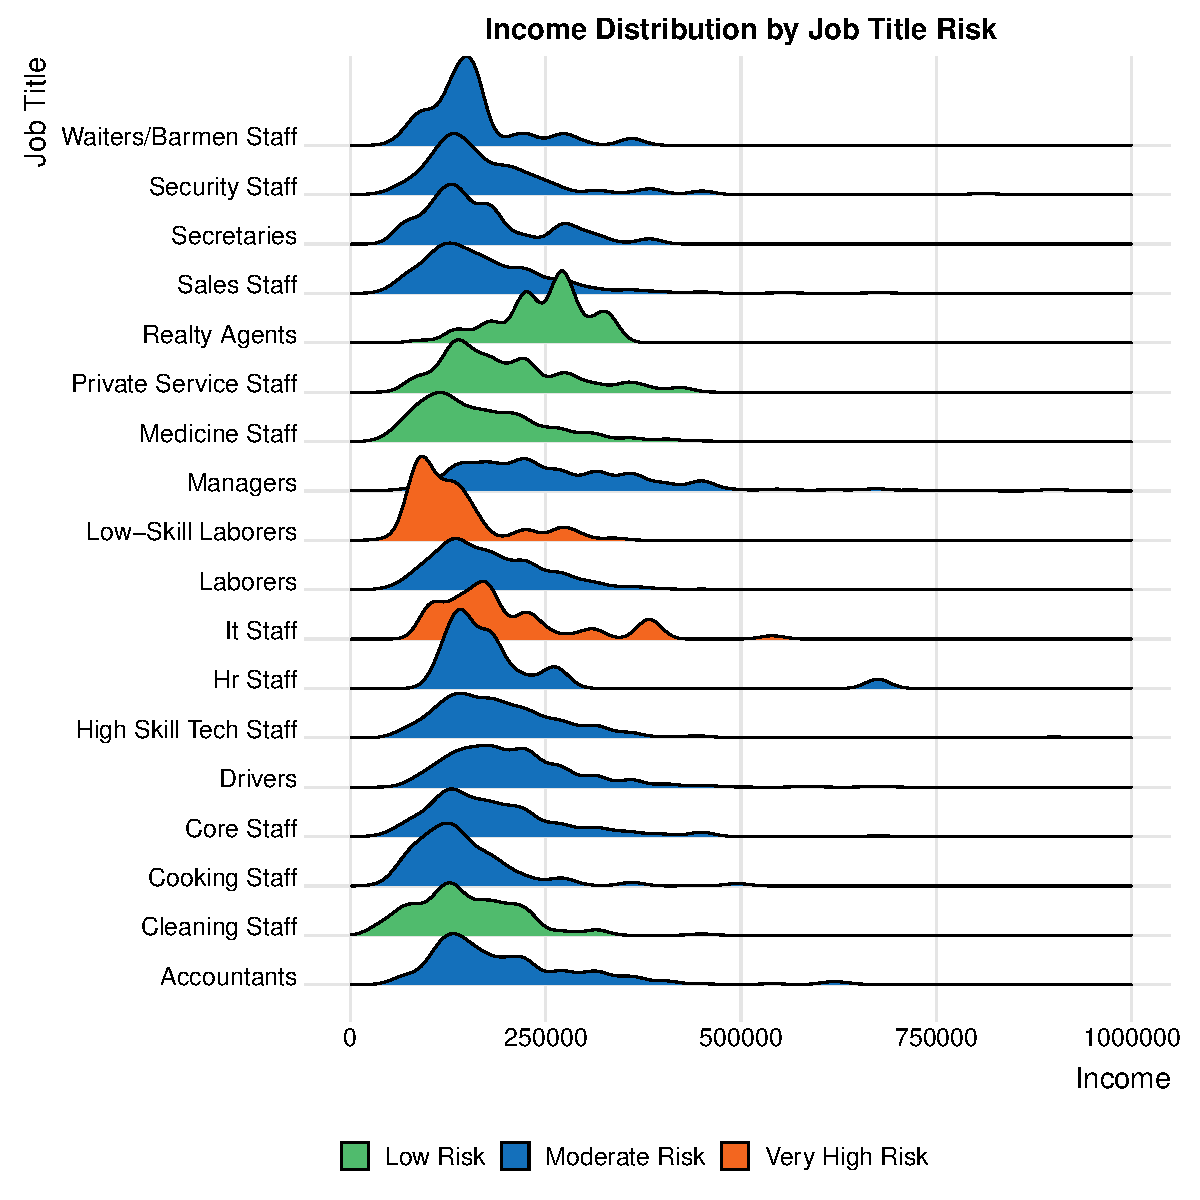
\includegraphics[width=\maxwidth]{figure/unnamed-chunk-45-1} \caption[Income by Job Title Risks]{Income by Job Title Risks}\label{fig:unnamed-chunk-45}
\end{figure}

\end{knitrout}

\subsubsection{Analysis and answer}

`It Staff' and `Low-Skill Laborers' job are at risk the most as compared with others. On the other hand, `Cleaning Staff', `Medicine Staff', `Private Service Staff' and `Realty Agents' jobs have low risk associated, with `Realty Agents' job being practically risk free. Moderate risk jobs has a wider range of incomes than the other two risk classes. It includes both high-income earners and those with lower incomes. In light of these information, `IT Staff' (4.6\%) and `Low-Skill Laborers' (5\%) includes a disproportionately high percentage of high-risk individuals, significantly higher than the average proportion of 1.7\% across moderate risk job titles and less than 1\% across low risk job titles.\\

Upon investigating their income pattern, it can be observed that jobs with highly skewed income distribution were high risk. Moderate risk jobs follow a similar normal distribution, while low risk jobs often have a more concentrated income range


\subsection{How does employment duration and status influence income levels among customers?}

\begin{knitrout}
\definecolor{shadecolor}{rgb}{0.969, 0.969, 0.969}\color{fgcolor}\begin{kframe}
\begin{alltt}
\hldef{percentile_90} \hlkwb{<-} \hlkwd{quantile}\hldef{(df}\hlopt{$}\hldef{Income,} \hlkwc{probs} \hldef{=} \hlnum{0.9}\hldef{)}

\hldef{t2.rect1} \hlkwb{<-} \hlkwd{data.frame}\hldef{(}
  \hlkwc{xmin} \hldef{=} \hlkwd{min}\hldef{(}\hlkwd{log}\hldef{(}\hlkwd{abs}\hldef{(df}\hlopt{$}\hldef{Employment.relative.length))),}
  \hlkwc{xmax} \hldef{=} \hlkwd{max}\hldef{(}\hlkwd{log}\hldef{(}\hlkwd{abs}\hldef{(df}\hlopt{$}\hldef{Employment.relative.length))),}
  \hlkwc{ymin} \hldef{= percentile_90,}
  \hlkwc{ymax} \hldef{=} \hlkwd{max}\hldef{(df}\hlopt{$}\hldef{Income)}
\hldef{)}

\hlkwd{ggplot}\hldef{(df,}
       \hlkwd{aes}\hldef{(}\hlkwc{x} \hldef{=} \hlkwd{log}\hldef{(}\hlkwd{abs}\hldef{(Employment.relative.length)),} \hlkwc{y} \hldef{= Income,}
           \hlkwc{shape} \hldef{= Employment.status,} \hlkwc{color} \hldef{= Employment.status))} \hlopt{+}
  \hlkwd{geom_rect}\hldef{(}\hlkwc{data} \hldef{= t2.rect1,}
            \hlkwd{aes}\hldef{(}\hlkwc{xmin} \hldef{= xmin,} \hlkwc{xmax} \hldef{= xmax,} \hlkwc{ymin} \hldef{= ymin,} \hlkwc{ymax} \hldef{= ymax),}
            \hlkwc{fill} \hldef{=} \hlsng{"#50bb6d"}\hldef{,} \hlkwc{alpha} \hldef{=} \hlnum{0.2}\hldef{,} \hlkwc{inherit.aes} \hldef{=} \hlnum{FALSE}\hldef{)} \hlopt{+}
  \hlkwd{geom_point}\hldef{(}\hlkwc{size} \hldef{=} \hlnum{0.6}\hldef{,} \hlkwc{alpha} \hldef{=} \hlnum{0.5}\hldef{)} \hlopt{+}
  \hlkwd{theme_classic}\hldef{()} \hlopt{+}
  \hlkwd{labs}\hldef{(}\hlkwc{x} \hldef{=} \hlsng{"Log of Absolute Employment Relative Length"}\hldef{,}
       \hlkwc{y} \hldef{=} \hlsng{"Income"}\hldef{,}
       \hlkwc{title} \hldef{=} \hlsng{"Relationship between Employment Duration and Income"}\hldef{)} \hlopt{+}
  \hlkwd{geom_hline}\hldef{(}
    \hlkwc{yintercept} \hldef{= percentile_90,} \hlkwc{linetype} \hldef{=} \hlsng{"dashed"}\hldef{,} \hlkwc{color} \hldef{=} \hlsng{"black"}\hldef{)} \hlopt{+}
  \hlkwd{annotate}\hldef{(}\hlsng{"text"}\hldef{,}
           \hlkwc{x} \hldef{=} \hlkwd{max}\hldef{(}\hlkwd{log}\hldef{(}\hlkwd{abs}\hldef{(df}\hlopt{$}\hldef{Employment.relative.length))),}
           \hlkwc{y} \hldef{= percentile_90,} \hlkwc{label} \hldef{=} \hlsng{"90th Percentile"}\hldef{,}
           \hlkwc{vjust} \hldef{=} \hlnum{1}\hldef{,} \hlkwc{hjust} \hldef{=} \hlnum{1.25}\hldef{,} \hlkwc{color} \hldef{=} \hlsng{"black"}\hldef{)} \hlopt{+}
  \hlkwd{annotate}\hldef{(}\hlsng{"text"}\hldef{,}
           \hlkwc{x} \hldef{=} \hlkwd{mean}\hldef{(}\hlkwd{log}\hldef{(}\hlkwd{abs}\hldef{(df}\hlopt{$}\hldef{Employment.relative.length))),}
           \hlkwc{y} \hldef{=} \hlkwd{mean}\hldef{(}\hlkwd{c}\hldef{(percentile_90,} \hlkwd{max}\hldef{(df}\hlopt{$}\hldef{Income))),}
           \hlkwc{label} \hldef{=} \hlsng{"High Income"}\hldef{,} \hlkwc{color} \hldef{=} \hlsng{"black"}\hldef{,} \hlkwc{size} \hldef{=} \hlnum{5}\hldef{,}
           \hlkwc{hjust} \hldef{=} \hlnum{3.5}\hldef{,} \hlkwc{vjust} \hldef{=} \hlopt{-}\hlnum{8}\hldef{)} \hlopt{+}
  \hlkwd{theme}\hldef{(}\hlkwc{plot.title} \hldef{=} \hlkwd{element_text}\hldef{(}\hlkwc{hjust} \hldef{=} \hlnum{0.5}\hldef{,} \hlkwc{face} \hldef{=} \hlsng{"bold"}\hldef{),}
        \hlkwc{legend.position} \hldef{=} \hlsng{"bottom"}\hldef{,}
        \hlkwc{legend.key.size} \hldef{=} \hlkwd{unit}\hldef{(}\hlnum{1.2}\hldef{,} \hlsng{"cm"}\hldef{))} \hlopt{+}
  \hlkwd{guides}\hldef{(}\hlkwc{color} \hldef{=} \hlkwd{guide_legend}\hldef{(}\hlkwc{override.aes} \hldef{=} \hlkwd{list}\hldef{(}\hlkwc{size} \hldef{=} \hlnum{4}\hldef{)))}
\end{alltt}
\end{kframe}\begin{figure}[H]
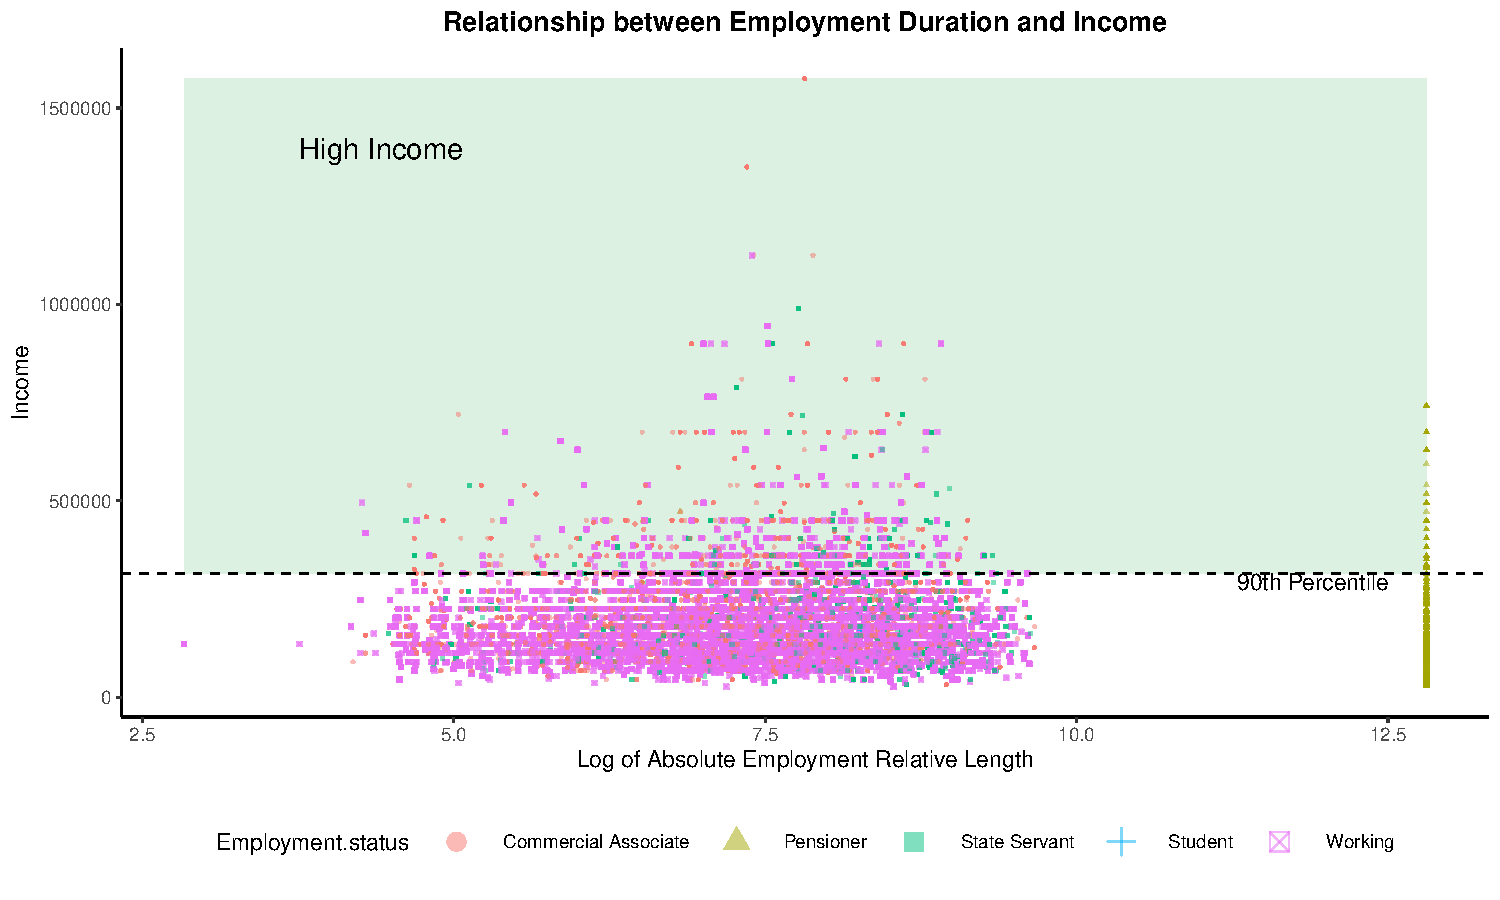
\includegraphics[width=\maxwidth]{figure/unnamed-chunk-46-1} \caption[Employment Duration and Income]{Employment Duration and Income}\label{fig:unnamed-chunk-46}
\end{figure}

\end{knitrout}

\subsubsection{Analysis and answer}

The findings suggests that employment status and duration are indeed important contributors to observed earnings differentials.  The majority of high-income individuals (defined as those earning above the 90th percentile) are concentrated in the `Commercial Associate' category. Other high income customers have employment status either `State Servant' or `Working'. \\

Furthermore, early years in career seem pretty key to broader earning opportunity later on, especially for those in `Commercial Associate' roles.  For those in `Working' status, employment duration is associated with income in a non-linear way with income increasing at first but showing a potential plateau or decline after a certain point. 


\subsection{Does asset ownership significantly impact income levels, and does this impact differ between high-risk and low-risk customers?}

\begin{knitrout}
\definecolor{shadecolor}{rgb}{0.969, 0.969, 0.969}\color{fgcolor}\begin{kframe}
\begin{alltt}
\hlkwd{ggplot}\hldef{(df,} \hlkwd{aes}\hldef{(}\hlkwc{x} \hldef{= Has.a.car,} \hlkwc{y} \hldef{= Income,} \hlkwc{color} \hldef{= Is.high.risk))} \hlopt{+}
  \hlkwd{geom_boxplot}\hldef{()} \hlopt{+}
  \hlkwd{facet_wrap}\hldef{(}\hlopt{~} \hldef{Has.a.property,}
             \hlkwc{labeller} \hldef{=} \hlkwd{as_labeller}\hldef{(}
               \hlkwd{c}\hldef{(}\hlsng{"TRUE"} \hldef{=} \hlsng{"Has Property"}\hldef{,} \hlsng{"FALSE"} \hldef{=} \hlsng{"No Property"}\hldef{)}
             \hldef{)}
  \hldef{)} \hlopt{+}
  \hlkwd{labs}\hldef{(}
    \hlkwc{x} \hldef{=} \hlsng{"Has Car"}\hldef{,}
    \hlkwc{y} \hldef{=} \hlsng{"Income"}\hldef{,}
    \hlkwc{title} \hldef{=} \hlsng{"Income Distribution by Risk Status, Property, and Car Ownership"}
  \hldef{)} \hlopt{+}
  \hlkwd{theme_classic}\hldef{()} \hlopt{+}
  \hlkwd{theme}\hldef{(}
    \hlkwc{legend.position} \hldef{=} \hlsng{"bottom"}\hldef{,}
    \hlkwc{legend.title} \hldef{=} \hlkwd{element_blank}\hldef{(),}
    \hlkwc{plot.title} \hldef{=} \hlkwd{element_text}\hldef{(}
      \hlkwc{hjust} \hldef{=} \hlnum{0.5}\hldef{,} \hlkwc{face} \hldef{=} \hlsng{"bold"}\hldef{,} \hlkwc{margin} \hldef{=} \hlkwd{margin}\hldef{(}\hlkwc{b} \hldef{=} \hlnum{10}\hldef{)))} \hlopt{+}
  \hlkwd{scale_color_manual}\hldef{(}
    \hlkwc{values} \hldef{=} \hlkwd{c}\hldef{(}\hlsng{"red"}\hldef{,} \hlsng{"blue"}\hldef{),} \hlkwc{labels} \hldef{=} \hlkwd{c}\hldef{(}\hlsng{"High Risk"}\hldef{,} \hlsng{"Low Risk"}\hldef{))}
\end{alltt}
\end{kframe}\begin{figure}[H]
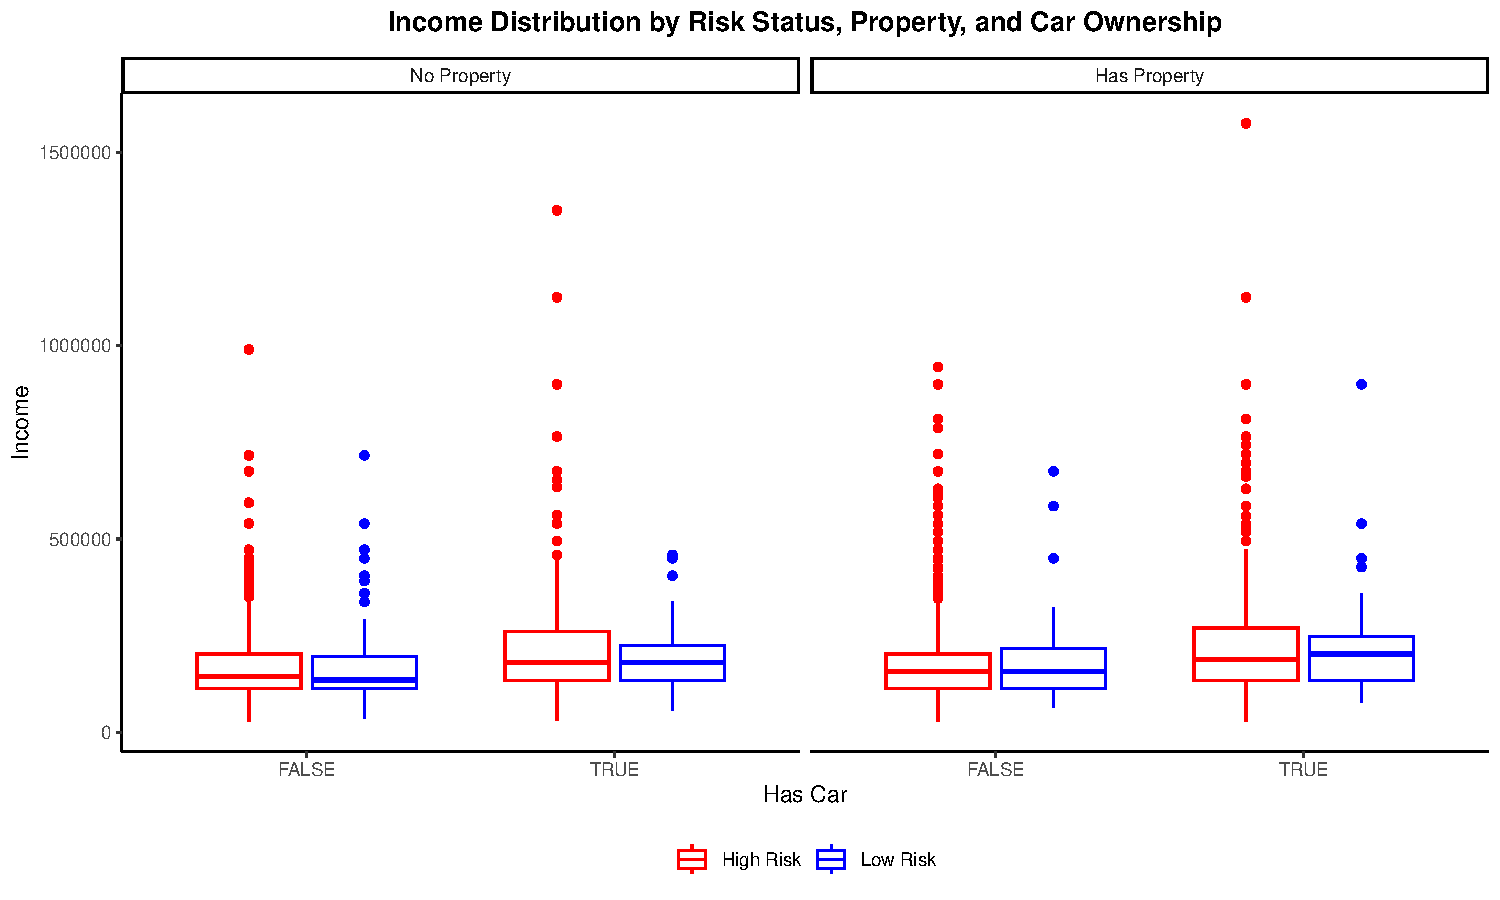
\includegraphics[width=\maxwidth]{figure/unnamed-chunk-47-1} \caption[Feature Importance for Classifying Customer Risk]{Feature Importance for Classifying Customer Risk}\label{fig:unnamed-chunk-47}
\end{figure}

\end{knitrout}

\subsubsection{Analysis and answer}

The results show a positive association between asset ownership and income. Customers who own property tend to have higher incomes than those without. In the same way car ownership indicates a higher income. These findings suggest that asset accumulation plays a role in influencing earning potential.\\

The study also identified a unique pattern for high-risk customers: higher and a highly skewed distribution of income. This means that even though people that are high-risk tend to earn more in total, their income levels are also more spread out with a good number of them having very high incomes.\\

To sum up, the results show a positive association between asset ownership and income, and high-risk customers exhibited a higher and more skewed income distribution, highlighting the need for targeted financial products that address income variability.



\subsection{Does higher education level mean high income?}

\begin{knitrout}
\definecolor{shadecolor}{rgb}{0.969, 0.969, 0.969}\color{fgcolor}\begin{kframe}
\begin{alltt}
\hlkwd{unique}\hldef{(df}\hlopt{$}\hldef{Education.level)}
\end{alltt}
\begin{verbatim}
## [1] "Secondary / Secondary Special" "Higher Education"             
## [3] "Incomplete Higher"             "Lower Secondary"              
## [5] "Academic Degree"
\end{verbatim}
\begin{alltt}
\hldef{education_order} \hlkwb{<-} \hlkwd{c}\hldef{(}\hlsng{"Lower Secondary"}\hldef{,} \hlsng{"Secondary / Secondary Special"}\hldef{,}
                     \hlsng{"Incomplete Higher"}\hldef{,} \hlsng{"Higher Education"}\hldef{,} \hlsng{"Academic Degree"}\hldef{)}

\hldef{median_income} \hlkwb{<-} \hldef{df} \hlopt
  \hlkwd{group_by}\hldef{(Education.level)} \hlopt
  \hlkwd{summarize}\hldef{(}\hlkwc{Median.Income} \hldef{=} \hlkwd{median}\hldef{(Income))}

\hlkwd{ggplot}\hldef{(median_income,}
       \hlkwd{aes}\hldef{(}
         \hlkwc{x} \hldef{=} \hlkwd{factor}\hldef{(Education.level,} \hlkwc{levels} \hldef{= education_order),}
         \hlkwc{y} \hldef{= Median.Income))} \hlopt{+}
  \hlkwd{geom_segment}\hldef{(}\hlkwd{aes}\hldef{(}\hlkwc{x} \hldef{=} \hlkwd{factor}\hldef{(Education.level,} \hlkwc{levels} \hldef{= education_order),}
                   \hlkwc{xend} \hldef{=} \hlkwd{factor}\hldef{(Education.level,} \hlkwc{levels} \hldef{= education_order),}
                   \hlkwc{y} \hldef{=} \hlnum{0}\hldef{,} \hlkwc{yend} \hldef{= Median.Income),}
               \hlkwc{color} \hldef{=} \hlsng{"steelblue"}\hldef{,} \hlkwc{linetype} \hldef{=} \hlsng{"dashed"}\hldef{,} \hlkwc{alpha} \hldef{=} \hlnum{0.5}\hldef{)} \hlopt{+}
  \hlkwd{geom_point}\hldef{(}\hlkwd{aes}\hldef{(}\hlkwc{size} \hldef{= Median.Income),} \hlkwc{color} \hldef{=} \hlsng{"#f3661f"}\hldef{)} \hlopt{+}
  \hlkwd{geom_text}\hldef{(}\hlkwd{aes}\hldef{(}\hlkwc{label} \hldef{= Median.Income),} \hlkwc{vjust} \hldef{=} \hlopt{-}\hlnum{1}\hldef{,} \hlkwc{size} \hldef{=} \hlnum{3}\hldef{)} \hlopt{+}
  \hlkwd{theme_classic}\hldef{()} \hlopt{+}
  \hlkwd{labs}\hldef{(}\hlkwc{title} \hldef{=} \hlsng{"Median Income by Education Level"}\hldef{,}
       \hlkwc{x} \hldef{=} \hlsng{"Education Level (Increasing)"}\hldef{,}
       \hlkwc{y} \hldef{=} \hlsng{"Median Income"}\hldef{)} \hlopt{+}
  \hlkwd{scale_x_discrete}\hldef{(}\hlkwc{labels} \hldef{=} \hlkwd{c}\hldef{(}\hlsng{"Lower Secondary"}\hldef{,} \hlsng{"Secondary"}\hldef{,}
                              \hlsng{"Incomplete Higher"}\hldef{,} \hlsng{"Higher Education"}\hldef{,}
                              \hlsng{"Academic Degree"}\hldef{))} \hlopt{+}
  \hlkwd{scale_y_continuous}\hldef{(}\hlkwc{labels} \hldef{= scales}\hlopt{::}\hldef{comma,}
                     \hlkwc{breaks} \hldef{=} \hlkwd{seq}\hldef{(}\hlnum{0}\hldef{,} \hlnum{300000}\hldef{,} \hlkwc{by} \hldef{=} \hlnum{50000}\hldef{),}
                     \hlkwc{limits} \hldef{=} \hlkwd{c}\hldef{(}\hlnum{0}\hldef{,} \hlnum{300000}\hldef{))} \hlopt{+}
  \hlkwd{theme}\hldef{(}
    \hlkwc{plot.title} \hldef{=} \hlkwd{element_text}\hldef{(}\hlkwc{hjust} \hldef{=} \hlnum{0.5}\hldef{,} \hlkwc{face} \hldef{=} \hlsng{"bold"}\hldef{,} \hlkwc{margin} \hldef{=} \hlkwd{margin}\hldef{(}\hlkwc{b} \hldef{=} \hlnum{10}\hldef{)),}
    \hlkwc{axis.title.x} \hldef{=} \hlkwd{element_text}\hldef{(}\hlkwc{margin} \hldef{=} \hlkwd{margin}\hldef{(}\hlkwc{t} \hldef{=} \hlnum{10}\hldef{)))}
\end{alltt}
\end{kframe}\begin{figure}[H]
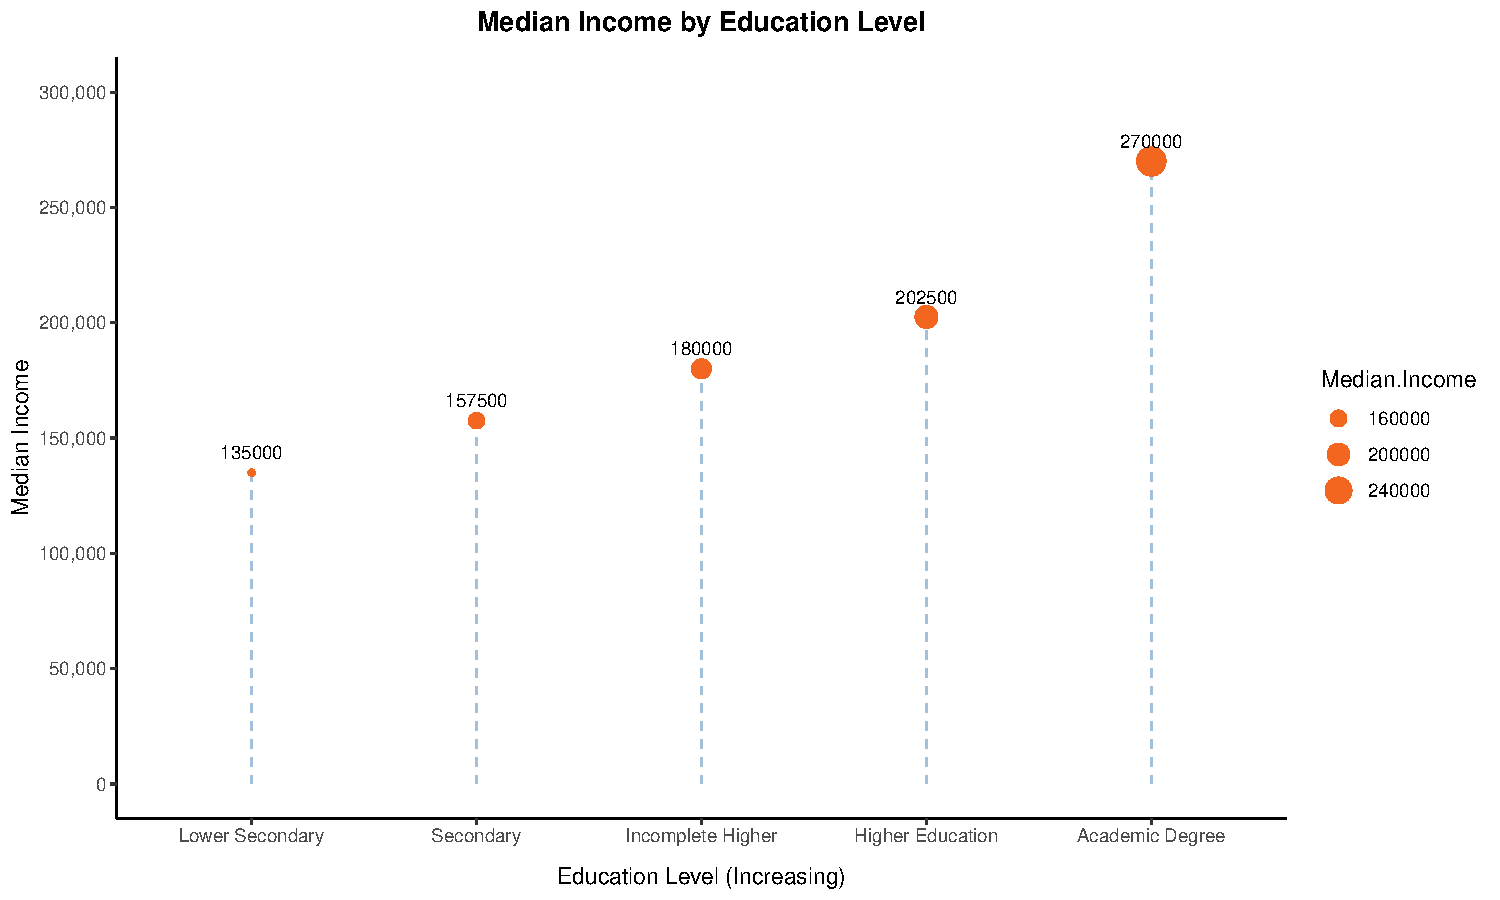
\includegraphics[width=\maxwidth]{figure/unnamed-chunk-48-1} \caption[Median Income by Customer Education Level]{Median Income by Customer Education Level}\label{fig:unnamed-chunk-48}
\end{figure}

\end{knitrout}

\subsubsection{Analysis and answer}

We see a positive correlation between education level and median income.It shows a strong upwards trend with an increase in median income with every higher level of educational attainment, from Lower Secondary to Academic Degree. Those having an Academic Degree make nearly the double the median income of those with Lower Secondary education. In other words, in the simplest of terms, it illustrates even more clearly that a higher educational attainment leads to a higher ability to earn, and supports the notion that education plays a crucial role in socioeconomic advancement.


\newpage
\section{Conclusion}

This report investigated the correlation of demographic and financials characteristics with the costumer credit risk using a comprehensive dataset named `Credit Card Eligibility Dataset'. The analysis was targeted to understanding the influence of employment status, education level, asset ownership, and income on credit risk as well as major factors effecting credit risk. Through data visualization techniques and predictive modeling, this study reveals significant correlations and trends, providing key insights on the intricate relationship between these variables and creditworthiness.\\

This analysis of the dataset highlights the significant role of several factors in determining customer credit risk. The report's findings to the non-trivial research questions include:\\

\begin{enumerate}

\item \begin{description}
\item[Q:] What factors greatly contribute to risk status of customers for credit card? 
\item[A:] Employment tenure and customer age have the strongest impact on risk status, followed by account age, income, and family member count respectively.\\
\end{description}

\item \begin{description}
\item[Q:] Which professions have a higher chance of being classified as high risk? 
\item[A:] Jobs in the categories `IT Staff' and `Low-Skill Laborers' have much higher odds of being deemed high-risk.\\
\end{description}

\item \begin{description}
\item[Q:] How does employment duration and status influence income levels among customers? 
\item[A:] Customers in mid-stage of career is the highest earning segment, with majority of high earners being `Commercial Associate' and `Working' status customers.\\
\end{description}

\item \begin{description}
\item[Q:] Does asset ownership significantly impact income levels, and does this impact differ between high-risk and low-risk customers? 
\item[A:] Yes, asset ownership significantly impacts income levels. High-risk customers with more assets tend to have higher income levels compared to low-risk customers with similar assets.\\
\end{description}

\item \begin{description}
\item[Q:] Does higher education level mean high income? 
\item[A:] Yes, higher education levels are strongly associated with higher median income.\\
\end{description}

\end{enumerate}

Similarly, the report highlights key findings about the customer distribution, including but not limited to:\\

\begin{enumerate}
\item Customer distribution show a predominant presence of males, married individuals, and customers with education levels typically up to Secondary/Secondary Special.
\item Most customers have 2 members in their family
\item Most customers have 0 children living.  
\item Most customers live in `House / Appartment' \\
\end{enumerate}

The dataset can be further explored to obtain additional findings. There is ample scope for asking more questions and performing deeper analysis to answer them using the dataset explored in this report.

\newpage
\addcontentsline{toc}{section}{References} % Add to the table of contents

\bibliographystyle{agsm} % Using the harvard citation style
\bibliography{references} % Including references from the .bib file

\end{document}
